\chapter{Continua}\label{chap:continua_Model}
Matters are composed of discrete objects such as molecules, yet studying macroscopic systems down to the discrete particles is challenging. For analytic purposes, it can be assumed that matters distributed \textit{continuously}  in many cases.  Continuum mechanics is the study of systems with such an assumption. This allows for studying the motion of macroscopic systems from fluids to solids without the need to model discrete underlying objects. The objective of the following section is to describe the fundamental principles of continua to the extent relevant in this manuscript.

\subsection*{Definitions}
Throughout section \S\ref{chap:continua_Model}, the following conventions are used to denote the quantities associated with continua. \textit{Scalar} (zero-rank tensor) variables are denoted by lower or upper case light face Latin and Greek letters, e.g., $\rho$ and $\phi$. Boldface lower case Latin letters, e.g. $\vect{u}$, are used to denote \textit{vectors} (first-order tensor) quantities. Boldface upper case Latin letters as well boldface lower case Greek letters, e.g. $\vect{E}$,  and $\bm \sigma$, are used for \textit{tensor} (second-order tensors) variables. Lastly, it is assumed that the problem is 3D and scalars, vectors, and tensors are comprised of 1, 3, and 9 elements, respectively. 

\section{Conservation Principles in Continua}
Conservation principles is an important aspect of continua as it allows studying the conserved variables such as mass, momentum, energy, and so forth.

In a given \textit{control volume} ($\mathbf{V}$) of a continuum surrounded by the control surface ($\mathbf{S}$), illustrated in Fig.~\ref{fig:CV}, a conserved value $\phi$ behaves such that :
\begin{figure}[H]
	\begin{center}
		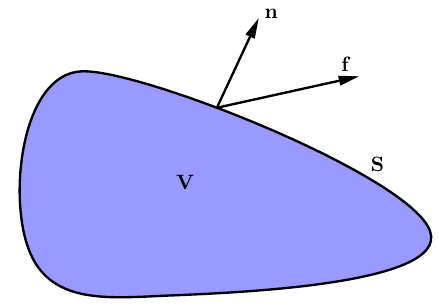
\includegraphics[width=.4\linewidth]{images/CV.png}
	\end{center}
	\caption{The control volume $\vect V$ bounded by the control surface $\vect S$. At every point on the control surface the vector $\vect {n}$ is pointing outward, and the $\vect{f}$ is the flux of a property that enter or exit the control volume.}
	\label{fig:CV}
\end{figure}
\begin{equation}
\parbox{4cm}{\centering the rate of change of $C$  in the control volume $\mathbf{V}$} = 
\parbox{4cm}{\centering the rate at which the $C$ enters or leave the domain through the control surface $\mathbf{S}$ } +
\parbox{4cm}{\centering the rate of generation or dissipation of $C$  inside the control volume $\mathbf{V}$}.  \label{eq:conservation}
\end{equation}
Assuming that $c=c(\vect{x},t)$ is the concentration of a scalar variable $C$ per unit mass of the control volume, $\phi(\vect{x},t)=\rho(\vect{x},t) c(\vect{x},t) $ is the concentration of $C$ per unit volume, and $\rho=\rho(\vect{x},t)$ is the density of the medium, it follows that:
\begin{equation}
C=\int_{V} c(\vect{x},t) dm= \int_{V} c(\vect{x},t) \rho(\vect{x},t) d{\vect{x}} = \int_{V} \phi (\vect{x},t) d{\vect{x}} .
\label{eq:Concentration}
\end{equation}
The flux of a variable is defined as the amount of the variable per unit area and unit time that enters or leaves ${V}$ through ${S}$. It follows from Eq.~\ref{eq:conservation} that
\begin{equation}
\frac{\partial}{\partial t} \int_{{V}} \phi (\vect{x},t) d{\vect{x}}= 
- \int_{{S}} \vect{f}(\vect{x},t) \bigcdot \vect{n} ds+
\int_{{V}} s (\vect{x},t) d{\vect{x}},
\label{eq:conservation_integral}
\end{equation}
which is the integral form of conservation law. After applying the divergence theorem 
\begin{equation}
\int_{{S}} \vect{f} \bigcdot \vect{n} ds=
\int_{{V}} (\nabla \bigcdot \vect{f})   d{\vect{x}},
\label{eq:divergence_theo}
\end{equation}
and assuming that the functions $\phi(\vect{x},t)$ and $\vect{f}(\vect {x},t)$ are differentiable and the divergence theorem holds, the \textit{differential form} of the conservation law is obtained as follows,
\begin{align}
\frac{\partial \phi (\vect{x},t) }{\partial t}  +
\nabla \bigcdot \vect{f}(\vect {x},t) 
-
s(\vect{x},t)=0.
\label{eq:conservation_differential}
\end{align}
The flux of $\phi$ comes from advection and diffusion of $\phi$ as follows:
\begin{align}
\vect{f}(\vect{x},t)=
\underbrace{\vect{u}(\vect{x},t) \phi(\vect{x},t)}_{\text{advection of $\phi$}} 
\underbrace{- \vect{D}(\vect{x},t) \nabla\phi(\vect{x},t)}_{\text{diffusion of $\phi$}},
\label{eq:Flux}
\end{align} 
where $\vect{D}$ is the diffusion matrix. Substituting the flux in Eq.~\ref{eq:conservation_differential} and dropping the space and time dependency for simplicity, the following general form of conservation law is obtained:
\begin{align}
\frac{\partial \phi  }{\partial t}  + \nabla \bigcdot (\vect{u} \phi - \vect{D}  \nabla \phi) -s=0.
\label{eq:transport_simple}
\end{align}
%Further simplifications to the advective flux is possible assuming an incompressible flow. After incorporating the mass conservation $\nabla\bigcdot \vect{u}=0$ and using the following identity 
%\begin{align}
%\nabla \bigcdot (\vect{u}\phi)=  \vect{u} \bigcdot \nabla\phi + \phi \nabla \bigcdot \vect{u},\label{eq:identity}
%\end{align}
%the form of advection-diffusion-reaction equation of a generic transport variable $\phi$  for \textit{incompressible flow} becomes
%\begin{align}
%\frac{\partial \phi}{\partial t}  + \vect{u} \bigcdot \nabla \phi  -\nabla \bigcdot (\vect{D}  \nabla \phi) -s=0
%\label{eq:transport2}
%\end{align}
%Note that the equivalent Lagrangian form of the equation condenses the advective term and the $\frac{\partial \phi}{\partial t}$ into the material derivative as explained in Eq.~\ref{eq:Material_Derivative} as follows:
%\begin{align}
%\frac{D \phi}{Dt}   -\nabla \bigcdot (\vect{D}  \nabla \phi) -s=0
%\label{eq:transport_lagrangian}
%\end{align}


\subsection{Mass Conservation}
Assume that $c=1$, i.e. $C$ is a \textit{scalar}  specifying the concentration of mass, and the integral in Eq.~\ref{eq:Concentration} is the physical \textit{mass} of the control volume. Substituting the $\phi=\rho c=\rho$ in Eq.~\ref{eq:conservation_differential} and assuming the advective flux vector of $\vect{f}=\vect{u} \phi= \rho \vect{u} $ and no mass source ($s=0$) leads to the generic forms of the continuity equation:
\begin{subequations}
	\begin{alignat}{3}
	\frac{\partial \rho }{\partial t}  + \nabla \bigcdot (\rho \vect{u} )=0 \label{eq:continuity_1},\\
	\frac{\partial \rho }{\partial t}  +\vect{u} \bigcdot \nabla\rho + \rho \nabla \bigcdot \vect{u}=0\label{eq:continuity_2},\\
	\frac{D \rho }{D t} + \rho \nabla \bigcdot \vect{u}=0 \label{eq:continuity_3}.
	\end{alignat}\label{eq:continuity}
\end{subequations}
The last equation is derived after incorporating the material derivative, 
\begin{align}
\frac{D(\;)}{Dt}&=\frac{\partial (\;)}{\partial t} + \vect{u} \bigcdot  \nabla(\;).  \label{eq:Material_Derivative}
\end{align}
Incompressible flow assumption ($D\rho/Dt=0$) may further simplify the mass conservation equations Eqs.~\ref{eq:continuity} to:
\begin{equation}
\nabla \bigcdot \vect{u}=0 \label{eq:continuity_incompressible}.
\end{equation}



\subsection{Momentum Conservation}
The conservation of momentum, also called Navier-Stokes equations, can be derived assuming that $c=\mathbf{u}$ and $\phi=\rho c=\rho \mathbf{u}$, i.e. $C$ is a vector specifying the momentum concentration. The flux tensor can be written as the sum of advective and stress flux, i.e. 
\begin{align}
\vect{f}=& \vect{u}(\vect{x},t) \phi(\vect{x},t) - \bm{\sigma}(\vect{x},t) =\rho\vect{u}\vect{u}-\bm\sigma \nonumber\\
=& \rho\begin{bmatrix}
u_1u_1& u_1u_2& u_1u_3\\
u_2u_1& u_2u_2& u_2u_3\\
u_3u_1& u_3u_2& u_3u_3\\
\end{bmatrix}+
\begin{bmatrix}
\sigma_{11}& \sigma_{12}& \sigma_{13}\\
\sigma_{21}& \sigma_{22}& \sigma_{23}\\
\sigma_{31}& \sigma_{32}& \sigma_{33}\\
\end{bmatrix},
\label{eq:mom_flux}
\end{align}
where $\vect{u} \vect{u}$ is a tensor results from the dyadic product of $\vect{u}$ by itself, and $\bm{\sigma}(\vect{x},t)$ is the stress flux. Substituting the flux tensor of Eq.~\ref{eq:mom_flux} in Eq.~\ref{eq:conservation_differential} results in the conservative Cauchy equations as follows
\begin{align}
\frac{\partial (\rho \vect{u})  }{\partial t}  + \nabla \bigcdot (\rho \vect{u} \vect{u} -  \bm \sigma) -s=\vect{0},
\label{eq:Momentum_Eu}
\end{align}
Further simplifications to the advective flux is possible assuming an incompressible flow. After incorporating the mass conservation $\nabla\bigcdot \vect{u}=0$ and using the following identity 
\begin{align}
\nabla \bigcdot (\vect{u}\phi)=  \vect{u} \bigcdot \nabla\phi + \phi \nabla \bigcdot \vect{u},\label{eq:identity}
\end{align}
with $\phi=\rho \vect{u}$ the second term can be simplified to 
\begin{align}\label{eq:non-conservative}
\nabla \bigcdot (\rho\vect{u}\vect{u})=\vect{u} \bigcdot \nabla(\rho\vect{u})+ \rho\vect{u} (\nabla \bigcdot \vect{u})=\vect{u} \bigcdot \nabla(\rho\vect{u}),
\end{align}
which subsequently can be used in conjunction with \ref{eq:Material_Derivative} to express the Cauchy equation in Lagrangian form as follows:
\begin{align}
\frac{ D (\rho \vect{u})  }{D t}  -\nabla \bigcdot  \bm \sigma -s=\vect{0}.
\label{eq:Momentum_La}
\end{align}

Note that Eq.~\ref{eq:non-conservative} simplifies the equations for a divergence-free velocity field. However, if the initial velocity field is not divergence-free, there will be error associated with ignoring this term at the initial time step.
 
Eqs.~\ref{eq:Momentum_Eu} and \ref{eq:Momentum_La} are respectively  Eulerian and Lagrangian momentum transport in any continuum. Further simplification requires more information about the nature of the continuum of interest. 
Conventionally in fluids and many other incompressible continua, $\bm{\sigma}$ can be decomposed into a volumetric (hydrostatic) part and a \textit{traceless} deviatoric part, as follows:
\begin{align}
&\bm{\sigma}=\bm{\sigma}^{dev}+\bm{\sigma}^{vol}\label{eq:stress_decomp},\\
&tr(\bm{\sigma}^{vol})=tr(\bm{\sigma})=\sigma_{11}+\sigma_{22}+\sigma_{33},\\
&tr(\bm{\sigma}^{dev})=0.
\end{align}
where $tr( )$ indicates sum of the diagonal elements of a tensor. Defining 
\begin{equation}
p=-({\sigma_{11}+\sigma_{22}+\sigma_{33}})/{3},\label{eq:stress_p}
\end{equation}
to be the mechanical pressure, the volumetric and the deviatoric parts of the stress tensor may be written as follows:
\begin{align}
&\bm{\sigma}^{vol}=(\frac{\bm{\sigma}: \mathbf{I}}{3}) \mathbf{I}=(\frac{\sigma_{11}+\sigma_{22}+\sigma_{33}}{3}) \mathbf{I}=
-p
\begin{bmatrix}
1& 0& 0\\
0&1&0\\
0&0&1\\
\end{bmatrix},\label{eq:sigma_vol}\\
&\bm{\sigma}^{dev}=\bm{\sigma}-(\frac{\bm{\sigma}: \mathbf{I}}{3}) \mathbf{I}=
\begin{bmatrix}
\sigma_{11}& \sigma_{12}& \sigma_{13}\\
\sigma_{21}& \sigma_{22}& \sigma_{23}\\
\sigma_{31}& \sigma_{32}& \sigma_{33}\\
\end{bmatrix}+
\begin{bmatrix}
p& 0& 0\\
0&p&0\\
0&0&p\\
\end{bmatrix}.
\label{eq:sigma_dev}
\end{align}
Ultimately, substituting the flux of Eq.~\ref{eq:mom_flux}  and stress decomposition of Eqs.~\ref{eq:stress_decomp}, \ref{eq:sigma_vol} and \ref{eq:sigma_dev}  into Eq.~\ref{eq:conservation_differential} leads to:
\begin{align}
\frac{\partial \rho \vect{u} }{\partial t}  + \nabla \bigcdot (\rho\vect{u}\vect{u}-\bm{\sigma}^{vol}-\bm{\sigma}^{dev})-\vect{f}_b=\vect{0},
\label{eq:Cauchy_momentum}
\end{align}
where $\vect{f}_b$ is the body force that acts as the source term $\vect{s}$ seen in \ref{eq:conservation_differential}. According to  
\begin{align}
\nabla \bigcdot (-\bm{\sigma}^{vol})=\nabla \bigcdot (p\mathbf{I})=\nabla p, 
\end{align}
the momentum conservation for Eulerian frameworks becomes:
\begin{align}
\frac{\partial (\rho \vect{u}) }{\partial t}  + \vect{u} \bigcdot \nabla(\rho\vect{u}) + \nabla p- \nabla \bigcdot \bm{\sigma}^{dev} - \vect{f}_b=\vect{0}.\label{eq:Cauchy_momentum_Eu}
\end{align}
After applying the material derivative (Eq.~\ref{eq:Material_Derivative}), the Lagrangian form of the momentum equation is obtained as follows:
\begin{align}
\frac{D (\rho \vect{u}) }{D t}  + \nabla p- \nabla \bigcdot \bm{\sigma}^{dev} - \vect{f}_b=\vect{0}.\label{eq:Cauchy_momentum_La}
\end{align}

\section{Material Modeling}
The momentum balance equations described in Eqs.~\ref{eq:Cauchy_momentum_Eu} and \ref{eq:Cauchy_momentum_La} express fewer equations than unknowns ($p, \vect{u}, \bm \sigma $) for a general continuum. Hence, material behavior may be used to introduce more equations for closure. In the following section, constitutive equations required for modeling the  $\nabla \bigcdot \bm{\sigma}^{dev} $ term for the continua of interest in this work are presented.
\subsection{Newtonian Model}\label{sec:Newtonian}
For Newtonian fluids, the deviatoric part of the stress tensor is related to the shear rate, through $\bm{\sigma}^{dev} = 2 \mu \bm E$, where $\mu$ is a constant representing the dynamic viscosity of the fluid and \textit{deformation-rate} tensor $\bm E$ is obtained from the velocity gradient tensor as follows,
\begin{align}
\bm E=\frac{1}{2}(\nabla\bf{u}+\nabla\bf{u}^T).
\label{eq:def_rate}
\end{align}
Above note that $\bm E$ is half of the \textit{strain-rate} tensor, $(\nabla\bf{u}+\nabla\bf{u}^T)$. Given that $\nabla \bigcdot \vect{u}=0$ for incompressible flows, the term $\nabla  \bigcdot \bm \sigma^{dev}$  may be simplified using the incompressible flow assumption as follows:
\begin{align}
\nabla  \bigcdot \bm \sigma^{dev}&=\nabla \bigcdot (\mu (\nabla\bf{u}+\nabla\bf{u}^T)) \nonumber\\
& = \mu \nabla \bigcdot (\nabla \vect{u}) + \mu \nabla (\nabla \bigcdot  \vect{u})\nonumber\\
& = \mu \nabla^2 \vect{u}
\label{eq:div_grad_u},
\end{align}
where 
\begin{align}
\nabla^2 = \dfrac{\partial^2}{\partial x^2}+\dfrac{\partial^2}{\partial y^2}+\dfrac{\partial^2}{\partial z^2}.
\label{eq:laplacian_op}
\end{align}
is the Laplacian operator.
Above, note that  divergence of a second-order tensor $\vect{S}$ is defined via $\nabla \bigcdot \bm \sigma = \sigma_{ki,i}\vect{e}_k$ as follows: 
\begin{align}
&\nabla \bigcdot \bm{S}= [\frac{\partial }{\partial x}, \frac{\partial }{\partial y},\frac{\partial }{\partial z}] \bigcdot
\begin{bmatrix}
S_{11}& S_{12}& S_{13}\\
S_{21}& S_{22}& S_{23}\\
S_{31}& S_{32}& S_{33}\\
\end{bmatrix}=
\begin{bmatrix}[1.5]
\dfrac{\partial S_{11}}{\partial x}+ \dfrac{\partial S_{12}}{\partial y}+ \dfrac{\partial S_{13}}{\partial z}\\
\dfrac{\partial S_{21}}{\partial x}+ \dfrac{\partial S_{22}}{\partial y}+ \dfrac{\partial S_{23}}{\partial z}\\
\dfrac{\partial S_{31}}{\partial x}+ \dfrac{\partial S_{32}}{\partial y}+ \dfrac{\partial S_{33}}{\partial z}
\end{bmatrix}.
\label{eq:div_S}
\end{align}
Furthermore, given that $\nabla \vect{u}=\nabla(u_ie_i)= (u_ie_i)_{,j}e_j=u_{i,j} {e}_i{e}_j$,  the velocity gradient tensor and its transpose are defined as follows 
\begin{align}
\nabla  \vect{u}=\nabla
\begin{bmatrix}
u_1\\
u_2\\
u_3\\
\end{bmatrix}=
&\begin{bmatrix}[1.5]
\dfrac{\partial u_1}{\partial x}& \dfrac{\partial u_1}{\partial y}& \dfrac{\partial u_1}{\partial z}\\
\dfrac{\partial u_2}{\partial x}& \dfrac{\partial u_2}{\partial y}& \dfrac{\partial u_2}{\partial z}\\
\dfrac{\partial u_3}{\partial x}& \dfrac{\partial u_3}{\partial y}& \dfrac{\partial u_3}{\partial z}
\end{bmatrix},\\
\nabla  \vect{u}^T=
&\begin{bmatrix}[1.5]
\dfrac{\partial u_1}{\partial x}& \dfrac{\partial u_2}{\partial x}& \dfrac{\partial u_3}{\partial x}\\
\dfrac{\partial u_1}{\partial 2}& \dfrac{\partial u_2}{\partial y}& \dfrac{\partial u_3}{\partial x}\\
\dfrac{\partial u_1}{\partial 3}& \dfrac{\partial u_3}{\partial z}& \dfrac{\partial u_3}{\partial x}
\end{bmatrix}.
\label{eq:gradU}
\end{align}

The final form of the momentum conservation described in Eqs.~\ref{eq:Cauchy_momentum_Eu}-\ref{eq:Cauchy_momentum_La} under incompressible flow assumption and Newtonian fluid model is then:  
\begin{subequations}
	\begin{alignat}{2}
	\frac{\partial \rho \vect{u} }{\partial t}  + \vect{u} \bigcdot \nabla(\rho\vect{u}) + \nabla p- \mu\nabla^2 \vect{u}-\vect{f}_b=\vect{0},\label{eq:NS_IN_Eulerian}\\
	\frac{D (\rho \vect{u})}{D t}  + \nabla p- \mu\nabla^2 \vect{u} -\vect{f}_b=\vect{0},\label{eq:NS_IN_Lagrangian}
	\end{alignat}
	\label{eq:NS_IN}
\end{subequations}
where Eq.~\ref{eq:NS_IN_Eulerian} is used in Eulerian frameworks and Eq.~\ref{eq:NS_IN_Lagrangian} is the Lagrangian counterpart obtained after condensing the first two terms of Eq.~\ref{eq:NS_IN_Eulerian} via the material derivative relation (Eq.~\ref{eq:Material_Derivative}).

The adimensionalized Navier-Stokes equations may be written as follows:
\begin{align}
\frac{D{\bf u}}{dt} & =-Eu \frac{\nabla p}{\rho}  + \frac{1}{Re} \nabla^{2} {\bf u}+ \frac{1}{Fr^2}{\bf f}^b \label{eq:NS_nondim} \; ,
\end{align}
where the Euler number, $Eu=\frac{p_0}{\rho_0 u_0^2}$, is the ratio of the pressure to inertia forces (or static pressure to dynamic pressure). The Reynolds number, $Re=\frac{\rho u_0 L_0}{\mu}$, may be seen as the ratio of inertia to viscous forces. Finally, the Froude number, $Fr=\frac{U_0}{\sqrt{g_0 L_0}}$, may be seen as the ratio of the inertia to body forces. From the inviscid fluid assumption made in this paper, $\mu=0$, the $\frac{1}{Re} \nabla^{2} {\bf u}$ term drops out of the equations and the momentum balance is the interplay of inertia, pressure and gravity/body force. In other words, the equations come down to the conservative Euler equations, where the relative significance of different terms are characterized by the magnitude $Fr$ and $Eu$ numbers.
\subsection{Non-Newtonian Model}\label{sec:NonNewtonian}
Contrary to Newtonian fluids where the viscosity is a constant, in non-Newtonian fluid models it depends on parameters such as yield stress, shear-rate, and so forth. Many models have been propose to capture shear thinning, shear-thickening, and yield stress. Amongst all the possible fluid models, the Herschel-BulklManey fluid is employed in the present work. Defining the shear stress and shear strain-rate from their underlying tensors, respectively according to
\begin{align}
& \tau = \sqrt{2 \boldsymbol{\bm{\sigma}}^{dev}_{ij} : \boldsymbol{\bm {\sigma}}^{dev}_{ij}}\label{eq:tau}\\
& \dot{\gamma} = \sqrt{2 {\boldsymbol E}_{ij} : {\boldsymbol E}_{ij}}\; \label{eq:gamma_dot},
\end{align}
the Herschel-Bulkley model describe the stress-strain relation via  
\begin{align}
& \tau = \tau_0+k\dot{\gamma}^n,
\label{eq:HB_t}
\end{align}
where $k>0$ is a consistency index, and $n$ is the flow index. Herschel-Bulkley model is a general model in that it allows modeling various fluid behaviors using a combination of $n$, and $k$ as illustrated in Fig.~\ref{fig:HB}. This includes shear thickening (dilatant), shear thinning (pseudoplastic), and Bingham plastic models.
\begin{figure}[H]
	\begin{center}
		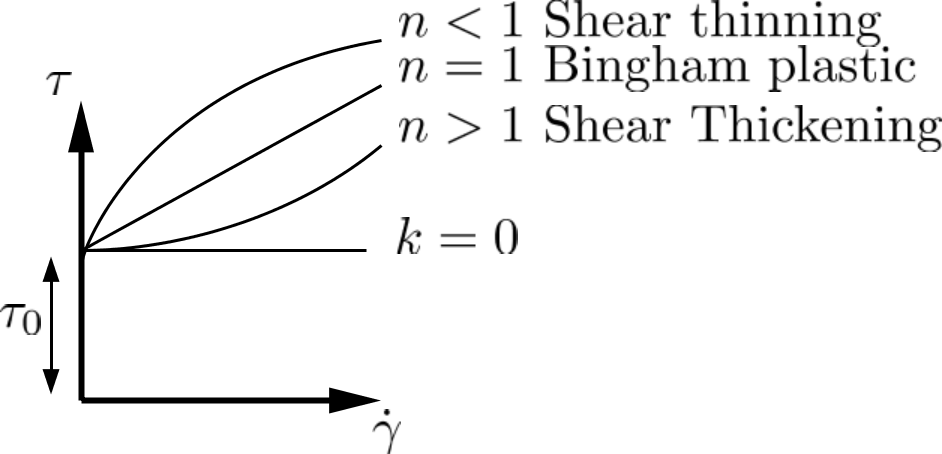
\includegraphics[width=.6\linewidth]{images/Non-newtonian.png}
	\end{center}
	\caption{Stress/strain-rate relationship for different flow index and consistency parameters in Herschel-Bulkley model \cite{ragui2018progress}.}
	\label{fig:HB}
\end{figure}
Subsequently, an apparent (effective) space-dependent viscosity satisfying $\tau = \mu_{eff}\dot{\gamma}$ and Eq.~\ref{eq:HB_t} may be defined \cite{WALLEVIK201495} as
\begin{align}
\mu_{eff}= \tau_0/\dot{\gamma}+k \dot{\gamma}^{n-1}.
\label{eq:HB_mu}
\end{align}
Finally, the deviatoric stress in the momentum balance is written as $\bm{\sigma}^{dev} = 2 \mu_{eff} \bm E$, where $\bm E$ is defined in Eq.~\ref{eq:def_rate}. Given the incompressible flow assumption the $\nabla  \bigcdot \bm \sigma^{dev}$ term in Eqs.~\ref{eq:Cauchy_momentum_Eu}-\ref{eq:Cauchy_momentum_La} is written as follows:
\begin{align}
\nabla  \bigcdot \bm \sigma^{dev}&=\nabla \bigcdot (\mu_{eff} (\nabla\bf{u}+\nabla\bf{u}^T)) \nonumber\\
& = \mu_{eff} \nabla \bigcdot (\nabla \vect{u}) 
+   \nabla \mu_{eff} \bigcdot \nabla \vect{u} 
+ \mu_{eff} \nabla (\nabla \bigcdot  \vect{u})
+ \nabla \mu_{eff}\bigcdot   \nabla  \vect{u}^T
\nonumber\\
& = \mu_{eff} \nabla^2 \vect{u}+   \nabla \mu_{eff} \bigcdot (\nabla \vect{u}+ \nabla  \vect{u}^T).
\label{eq:div_grad_u_NN}
\end{align}
The final form of the momentum balance for non-Newtonian fluids in Eulerian and Lagrangian frameworks respectively is as follows:
\begin{subequations}
	\begin{alignat}{2}
	\frac{\partial \rho \vect{u} }{\partial t}  + \vect{u} \bigcdot \nabla(\rho\vect{u}) + \nabla p- \mu_{eff}\nabla^2 \vect{u}-
	\nabla \mu_{eff} \bigcdot (\nabla \vect{u}+ \nabla  \vect{u}^T)
	-\vect{f}_b=\vect{0},\label{eq:NSE_Eulerian_NN}\\
	\frac{D (\rho \vect{u})}{D t}  + \nabla p- \mu_{eff}\nabla^2 \vect{u}
	-\nabla \mu_{eff} \bigcdot (\nabla \vect{u}+ \nabla  \vect{u}^T)
	-\vect{f}_b=\vect{0}.\label{eq:NSE_Lagrangian_NN}
	\end{alignat}
	\label{eq:NSE_NN}
\end{subequations}

\subsection{Granular Material}\label{sec:granular_material}
Proper continuum rheological models allows for applying Eqs.~\ref{eq:Cauchy_momentum_Eu} and \ref{eq:Cauchy_momentum_La} to granular materials. Amongst those, the $\mu(I)$ rheology \cite{daCruz2005} and the three-dimensional extension proposed in \cite{jop2006constitutiveNature} have been applied successfully in many works. The non-local rheology proposed in \cite{kamrinNonlocal2012} improves the rate-independent Drucker-Prager and Mohr-Coulomb model for dense and rapid granular flows.

In the present work, a rigid-plastic assumption is made. This assumption neglects the elastic response of the grains and approximates all flow as plastic flow. A similar strategy was employed in an Eulerian framework in \cite{lagree2011granular}. Another fundamental assumption made herein is to neglect the small variation of the volume fraction observed in the dense regime and describe granular material as an incompressible fluid \cite{jop2006constitutiveNature,kamrin2017hierarchy}. Following the stress decomposition described in Eqs.~\ref{eq:stress_decomp}, \ref{eq:stress_p}, \ref{eq:sigma_vol}, and \ref{eq:sigma_dev}, the deviatoric part of the stress tensor in the momentum balance Eq.~\ref{eq:Cauchy_momentum_La} is written similar to the non-Newtonian fluid model described in \S\ref{sec:NonNewtonian} as 
\begin{equation}
\bm{\sigma}^{dev} = 2 \mu_{eff} \bm E, \label{eq:stress_strainrate}
\end{equation}
where $\bm E$ is defined in Eq.~\ref{eq:def_rate}. This assumption about the codirectionality of the stress and strain-rate tensors neglects the presence of anisotropy that causes the eigenvectors of stress and strain-rate to misalign \cite{kamrin2017hierarchy}. The effective viscosity of granular material has been described via 
\begin{equation}
\mu_{eff}=\frac{\mu_g p}{\dot{\gamma} },
\end{equation}
in many previous works \cite{jop2006constitutiveNature}, where $\mu_g$ is used to denote the granular material friction coefficient, and $\dot{\gamma}$ and $p$ are defined from Eqs.~\ref{eq:gamma_dot} and \ref{eq:stress_p}, respectively. Subscript $g$ is used to distinguish the friction coefficient in granular medium, $\mu_g$, from the fluid viscosity $\mu$. 

The aforementioned description of the $\mu_{eff}$ is a special variance of the non-Newtonian model described by Eq.~\ref{eq:HB_mu}, 
\begin{equation*}
\mu_{eff}= \tau_0/\dot{\gamma}+k \dot{\gamma}^{n-1},
\end{equation*}
for $k=0$ and $\tau_0=\mu_g p$. The choice of $\mu_g p$ for the yield stress $\tau_0$ stands to the following rational. Consider the mass-spring-damper system shown in Fig.~\ref{fig:MSD}. Writing the force balance for the system as
\begin{align}
m \ddot{x} = -k x + -c \dot{x} - \mu_g F_n,
\end{align}
and dividing both sides by the contact area $A$, it follows that:
\begin{align}
\frac{m}{A} \ddot{x} =& -\frac{k}{A} x + -\frac{c}{A}\dot{x} - \mu_g \frac{F_n}{A}, \nonumber\\
\frac{m}{A} \ddot{x} =& 
-\underbrace{k^{\prime} x}_{\textbf{Elasticity}}
-\underbrace{c^{\prime} \dot{x}}_{\textbf{Viscosity}}
-\underbrace{\mu_g p}_{\textbf{Frictional contact}}.
\end{align}
\begin{figure}[H]
	\begin{center}
		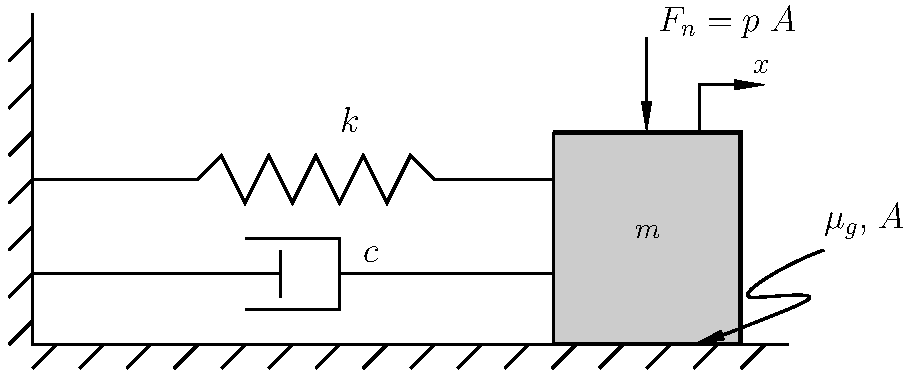
\includegraphics[width=.5\linewidth]{images/Mass_Spring_Damper.pdf}
	\end{center}
	\caption{A mass-spring-damper system consisting of viscous, elastic, and frictional resistive forces.}
	\label{fig:MSD}
\end{figure}

Accordingly, the relationship between elastic, viscous and frictional stresses may be seen as follows. The viscous stress is related to rate of deformation ($c^{\prime}\dot{x}$ and Eq.~\ref{eq:stress_strainrate}), while frictional contact causes a yield stress below which no motion happens. Hence, the choice of $\tau_0=\mu_g p$ in Eq.~\ref{eq:HB_mu} (see also Fig.~\ref{fig:HB}) is justified. Thus, the continuum modeling of granular material is performed as a special case of non-Newtonian fluids. 

\section{Time Integration}
In this section the main ideas behind the time integration of the continuum equations discussed in previous sections are described. The time-integration discussed herein are not tied to the choice of space discretization and are common among various Eulerian and Lagrangian CFD solvers. These integration schemes are employed in the I2SPH method that will be described in section \S\ref{sec:ISPH}.

\subsection{Projection Method}
This algorithm is based on the Helmholtz-Hodge decomposition, which states that any vector field $\vect{u}$ may be decomposed into a  solenoidal ($\vect{u}_{sol}$) and an irrotational ($\vect{u}_{irrot}$) part as follows:
\begin{equation}
\vect{u}=\vect{u}_{irrot}+\vect{u}_{sol},
\end{equation}
where the solenoidal part is divergent-free ($\nabla. \vect{u}_{sol}=0$). The irrotational part is curl-free ($\nabla \times \vect{u}_{irrot=0}$) and can be written as the gradient of a potential/scalar field ($\vect{u}_{irrot}=\nabla \phi$). The irrotational part is a conservative vector field, and the line integral of this field is path-independent.   
By taking divergence of $\vect u$ and using the divergent-free property of $\vect{u}_{sol}$, it can be seen that 
\begin{equation}\label{eq:phi_Poisson}
\nabla \bigcdot  \vect{u}=\nabla \bigcdot \vect{u}_{irrot}= \nabla^2 \phi,
\end{equation}
and given that $\vect{u}$ is known, the Poisson equation \ref{eq:phi_Poisson} can be solved for $\phi$ which finally results in $\vect{u}_{sol}=\vect{u} -\vect{u}_{irrot}=\vect{u}-\nabla \phi$.

In a similar fashion, we can decompose the force field per unit mass ($\dfrac{D{\vect u}}{Dt}$)  of Equation \ref{eq:NS_IN_Lagrangian} into a solenoidal field ($ \nu \nabla^{2} {\vect u}+{\vect{f}_b}$) and an irrotational field ($-\dfrac{1}{\rho} \nabla p$). The semi-discrete form (discretized only in time) of Eq.~\ref{eq:NS_IN_Lagrangian} is written as follows:
\begin{equation}
\dfrac{(\vect{u}^{n+1}-\vect{u}^n)}{\Delta t}= 
\underbrace{\dfrac{(\vect{u}^{n+1}-\vect{u}^*)}{\Delta t}}_{ \text{  solenoidal contribution}} 
+
\underbrace{\dfrac{(\vect{u}^{*}-\vect{u})}{\Delta t}}_{\text{ irrotational contribution}} = -\dfrac{1}{\rho} \nabla p +\nu \nabla^2\vect{u}^n + \vect{g}.
\end{equation}

\subsection{Non-Incremental Projection Method}
Based on the previous discussion the following decomposition is conducted: 
\begin{align}
\dfrac{(\vect{u}^*-\vect{u}^n)}{\Delta t}=&+\nu \nabla^2\vect{u}^n + \vect{g}=\vect{f}^n \quad x\in \Omega, \qquad \vect{u}^*=0 \quad x\in \partial\Omega,\label{eq:predict_HH} \\
\dfrac{(\vect{u}^{n+1}-\vect{u}^*)}{\Delta t}=&-\dfrac{1}{\rho} \nabla p^{n+1}\quad x\in \Omega, \qquad \nabla.\vect{u}^{n+1}=0 \quad \in \partial\Omega \label{eq:correct_HH}.
\end{align}
Eq.~\ref{eq:predict_HH} is the predictor step and it can be used to find the intermediate velocity $\vect{u}^*$:
\begin{equation}\label{eq:u_star}
\vect{u}^*=\vect{f}^n {\Delta t}+\vect{u}^n.
\end{equation}
Moreover, if pressure is known, Eq.~\ref{eq:correct_HH} may be used to find $\vect{u}^{n+1}$ as follows
\begin{equation}\label{eq:u_new}
\vect{u}^{n+1}=-{\Delta t}\dfrac{1}{\rho} \nabla p^{n+1}+\vect{u}^*.
\end{equation}
In order to obtain the pressure equation, using the approach led to Eq.~\ref{eq:phi_Poisson}, we take divergence of the Eq.~\ref{eq:correct_HH} and obtain the Poisson equation for pressure. 
\begin{equation}\label{eq:del_2p_HH}
\dfrac{\nabla \bigcdot \vect{u}^{n+1}-\nabla \bigcdot \vect{u}^*}{\Delta t}=-\dfrac{1}{\rho} \nabla^2 p^{n+1}.
\end{equation}
Note that from continuity Eq.~\ref{eq:continuity_1} with incompressible flow assumption $\dfrac{D\rho}{Dt}=0$ we can write  $\nabla \bigcdot \vect{u}^{n+1} =0$ and simplify Eq.~\ref{eq:del_2p_HH} to 
\begin{equation}\label{eq:pressure_1}
\dfrac{1}{\rho} \nabla^2 p^{n+1}=\dfrac{\nabla \bigcdot \vect{u}^*}{\Delta t}, \quad \nabla p^{n+1}\bigcdot\vect{n}|_{\partial \Omega}=0.
\end{equation}
Next, Eq.~\ref{eq:u_new} is used to update the velocities. The algorithm described above, \textit{velocity-based projection}, is usually preferred when the density variation is small and $\frac{D\rho}{Dt}=0$ holds. For Lagrangian methods such as SPH, when working with free-surface flows, the \textit{density-based projection} method is considered to be more accurate. In this method, the continuity equation is used to replace the velocity divergence term $\dfrac{\nabla\bigcdot \vect{u}^*}{\Delta t}$ in Eq.~\ref{eq:pressure_1}. The semi-discrete continuity equation is as follows
\begin{equation}\label{eq:cont_desc}
\dfrac{\rho^*-\rho^n}{\Delta t}=-\rho^n \nabla \bigcdot \vect{u}^*.
\end{equation}
Using the right hand side of \ref{eq:cont_desc}, one may write  Eq.~\ref{eq:pressure_1} as follows:
\begin{equation}\label{eq:pressure_2}
\dfrac{1}{\rho} \nabla^2 p^{n+1}=-\dfrac{1}{\rho^n}\dfrac{\rho^*-\rho^n}{\Delta t^2},
\end{equation}
which takes into consideration the density variation as a source term in the Poisson equation.\\


Another important aspect of the discretization of Eq.~\ref{eq:predict_HH} has to do with the treatment of the viscous forces. This discretization may be chosen to be explicit, implicit or semi-implicit in terms of $\vect{u}^*$  as follows:    
\begin{equation}
\dfrac{(\vect{u}^*-\vect{u}^n)}{\Delta t}=+\nu(\theta \nabla^2\vect{u}^* + (1-\theta)\nabla^2\vect{u}^n)+ \vect{g}=\vect{f}^n\label{eq:CN}.
\end{equation}
Eq.~\ref{eq:CN} corresponds to the fully-explicit scheme (E~\ref{eq:predict_HH}) for $\theta=0$, and to fully-implicit scheme for $\theta=1$. Crank-Nicolson discretization is obtained via $\theta=0.5$.

\subsection{Incremental Projection Method}
The incremental projection method with the Crank-Nicolson correction applied to the prediction step is as follows:
\begin{align}
\dfrac{(\vect{u}^*-\vect{u}^n)}{\Delta t}=&\frac{\nu}{2}(\nabla^2\vect{u}^* +\nabla^2\vect{u}^n) -\dfrac{1}{\rho} \nabla p+ \vect{g}=\vect{f}^n\label{eq:CN_2},\\
\dfrac{(\vect{u}^{n+1}-\vect{u}^*)}{\Delta t}=&-\dfrac{1}{\rho} (\nabla p^{n+1}-\nabla p^{n} )=-\dfrac{1}{\rho} (\nabla \phi ) \label{eq:correct_inc},\\
\phi=&p^{n+1}-p^{n}.
\end{align}
Herein, the Poisson equation is solved for $\phi$ instead of $p^{n+1}$. On an Eulerian grid, the pressure correction is performed via $p^{n+1}=p^{n}+\phi$, whereas in the Lagrangian methods the pressure correction is as follows:
\begin{equation}
p^{n+1}=p^{n}+\phi +\nabla p^{n+1}\bigcdot(\vect{x}^{n+1}-\vect{x}^{n}).
\end{equation}
See \cite{Trask2ndOrder2015,Hosseini2011} for more details about the advantages of the incremental projection method over the non-incremental variation.

\section{Space Discretization}\label{sec:Space-Discretization}
Given the problems of interest in the present work, we choose to employ a Lagrangian discretization method for spatial discretization of the governing equations of continua (Eqs.~\ref{eq:continuity} and \ref{eq:Cauchy_momentum_La}). Amongst possible choices of the Lagrangian methods, we choose the Smoothed Particle Hydrodynamics method as it has been studied quite extensively in the literature for the Navier-Stokes equations.
 
\subsection {Smoothed Particle Hydrodynamics}\label{sec:SPH}
The SPH  approximation of a function $f$ at location $\mathbf r_i$ as \cite{Monaghan2005a}
\begin{equation}\label{eq:SPH_f}
f(\mathbf r_i) \approx  \langle f\rangle_i= \sum_{j \in \support{i}} \frac{m_j}{\rho_j}f(\mathbf r_j)W_{ij} \; ,
\end{equation}
where $\langle f \rangle_i$ indicates the SPH approximation of $f$ at the location of SPH particle, or marker, $i$;  $\support{i}$ represents the collection of SPH particles found in the support domain associated with particle $i$; $\rho_j$ is the density $\rho({\bf r}_j)$ at location ${\bf r}_j$ of particle $j$; $m_j=\rho_j V_j$ and $V_j=(\sum_{k \in {\cal S}(j)} W_{jk})^{-1}$ are the mass and volume associated with marker $j$, respectively; $W_{ij}\equiv W(|\br_i-\br_j|,h)$, where $|{\bf r}|$ is the length of ${\bf r}$. The kernel function $W$ can assume various expressions, e.g., a cubic spline kernel for 3D problems:
\begin{equation} 
\label{eq:kernelExample}
W(|\br|,h) = \frac{5}{{14\pi {h^3}}} \times \left\{ \begin{aligned}
&{(2 - q)^3} - 4{(1 - q)^3}, && 0 \le q < 1 \\ 
&{(2 - q)^3}, && 1 \le q < 2 \\ 
&0, && q \ge 2 \\ 
\end{aligned} \right.,
\end{equation}
where, if the kernel function is located at the origin, $q\equiv | \mathbf{r} | / h$.  The radius of the support domain, $\kappa h$, is proportional to the characteristic length $h$ through the parameter $\kappa$, the latter commonly set to $2$ for the cubic spline kernel as shown in Fig.~\ref{fig:SPH}.
\begin{figure}[H]
	\begin{center}
		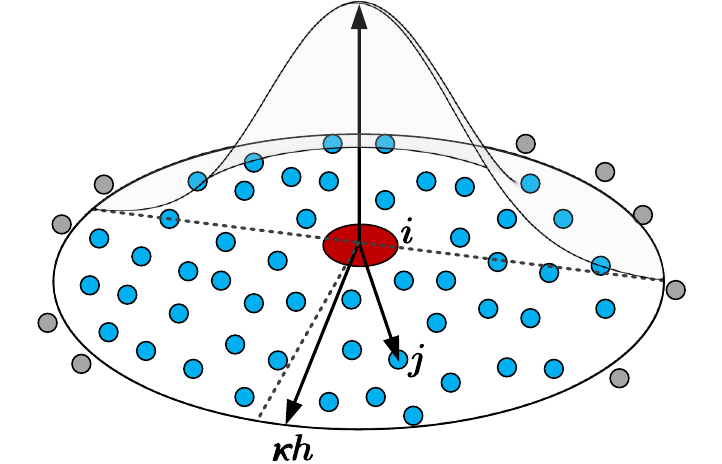
\includegraphics[width=.5\linewidth]{images/sph_kernel.png}
	\end{center}
	\caption{2D illustration of the kernel $W$. The radius of the support domain is defined as a multiple, $\kappa$, of the kernel's characteristic length, $h$.}
	\label{fig:SPH}
\end{figure}


The standard SPH gradient and Laplacian approximations assume the following expressions, respectively \cite{Monaghan2005a}:
\begin{align}
&\nabla f(\mathbf r_i) \approx \langle \nabla f \rangle_i=\sum_{j \in \support{i}} V_j (f_j-f_i) \nabla_i W_{ij}\label{eq:Standard_G},\\
&\nabla^2 f(\mathbf r_i) \approx \langle \nabla^2 f \rangle_i=2\sum_{j \in \support{i}} V_j ( \mathbf{e}_{ij} \cdot \nabla_i W_{ij}) \frac{f_i-f_j}{|\mathbf{r}_{ij}|} \; , \label{eq:Standard_L}
\end{align}
where $\mathbf{e}_{ij}=\dfrac{\mathbf{r}_{ij}}{|\mathbf{r}_{ij}|}$ and $\nabla_i$ denotes differentiation in space with respect to the coordinates of SPH particle $i$; i.e., 
\begin{equation}
\label{eq:nablaW}
\nabla_i W_{ij} =\left.\frac{\mathbf r_{ij}}{|\mathbf r_{ij}|} \frac{\partial W}{\partial q} \frac{\partial q}{\partial |\mathbf r_{ij}|}\right\vert_{i,j} =  \frac{-15{\mathbf r}_{ij}}{{14\pi {h^5}q}} \times \left\{ \begin{aligned}
&{(2 - q)^2} - 4{(1 - q)^2}, && 0 \le q < 1 \\ 
&(2 - q)^2, && 1 \le q < 2 \\ 
&0, && q \ge 2 \\ 
\end{aligned} \right.\; .
\end{equation}
%For simplicity, in what follows, $\nabla_i W_{ij}$ is replaced by $\nabla W_{ij}$. 

Elaborating on the concept of convergence and accuracy, if a numerical discretization matches the first $m$ terms of the Taylor expansion of the solution, then the numerical approximation
is said to be $(m + 1)^{th}$-order accurate and $\mathcal{C}^m$ consistent. The standard SPH discretizations have $\mathcal{C}^1$  consistency (exact approximation of linear functions) in the interior of the domain provided a regular particle distribution is maintained. If the particle regularity is lost over time, the standard discretization is no longer $\mathcal{C}^1$ consistent and corrections are required in order to maintain the consistency order. However, once the kernel function is altered to retain consistency, the SPH discretization will forfeit its symmetry attributes thus losing its conservation trait. Whereas conservative schemes are essential for the discretization of the pressure gradient term and pressure-driven flows, consistent schemes play a more important role in viscous flows. One side effect of using a consistent discretization is that it requires smaller kernel support \cite{Trask2015,islam2018consistency}. Reducing the support size and thus the number of neighbors is more critical in implicit solvers since linear system fill-in is dictated by the number of SPH particle neighbors. This is the rationale for using a consistent formulation for the implicit SPH method discussed herein, see \S\ref{sec:ISPH}, whenever handling an interior flow scenario.


\noindent The ``consistent'' discretization already defined for the conservative case in Eqs.~\ref{eq:Standard_G} and~\ref{eq:Standard_L} assumes the expression \cite{fatehi2011,randles1996}
\begin{align}
&\nabla f(\mathbf r_i) \approx \langle \nabla f \rangle_i=\sum_{j \in \support{i}} V_j (f_j-f_i)\; \mathbf{G}_i\; \nabla_i W_{ij},\label{eq:Consistent_G}\\
&\nabla^2 f(\mathbf r_i) \approx \langle \nabla^2 f \rangle_i=2\sum_{j \in \support{i}}  \left[ \mathbf{L}_i \;:\;  (\mathbf{e}_{ij} \otimes \nabla_i W_{ij}) \right] \Bigg( \frac{f_i-f_j}{|\mathbf{r}_{ij}|}  - \mathbf{e}_{ij} \cdot \nabla f_i\Bigg) V_j,\label{eq:Consistent_L}
\end{align}
where ``$\otimes$" represents the dyadic product of the two vectors; ``$:$" represents the double dot product of two matrices; and $\mathbf{G}_i$ and $\mathbf{L}_i$ are  second-order, symmetric correction tensors. The  $(m,n)$ element of the inverse of $\mathbf{G}_{i}$ is expressed as \cite{Libersky1993,randles1996,fatehi2011}: 
\begin{equation}\label{eq:gradient_Gi}
(\textbf{G}_{i}^{-1})^{mn}=-\sum\limits_j r_{ij}^{m}\nabla_{i,n}W_{ij}V_{j} \;.
\end{equation}
\noindent The $3 \times 3$ matrix $\mathbf{L}_i$ is symmetric and has six unknowns obtained as the solution of a linear system \cite{fatehi2011}. The required six independent equations may be obtained by expanding the following equation for the upper/lower triangular elements of a $3 \times 3 $ matrix, e.g. $m=1,n=1,2,3$,   $m=2,n=2,3$, and $m=3,n=3$.
\begin{equation}\label{eq:delta_mn}
-\delta^{mn}=\sum\limits_j(A_{i}^{kmn}e_{ij}^{k}+r_{ij}^{m}e_{ij}^{n})(L_{i}^{op}e_{ij}^{o}\nabla_{i,p}W_{ij}V_{j}) \; ,
\end{equation}
where $\delta^{mn}$ is the Kronecker symbol, and the elements of the third order tensor $A_{i}$ are obtained as 
\begin{equation}\label{equ:Ai_kmn}
A_{i}^{kmn}=\sum\limits_j r_{ij}^{m} r_{ij}^{n}G_{i}^{kq}\nabla_{i,q}W_{ij}V_{j} \;.
\end{equation}
A detailed account of obtaining the elements $\textbf{L}_i$ is provided in \cite{TR-2016-14}. 

The outcome of the SPH discretization steps described above can be conveniently represented in matrix form. To that end, at the beginning of a time step one computes and stores the discretization matrices $\mathbf{A}^G$ and $\mathbf{A}^L$ that arise from either the standard discretization Eqs.~\ref{eq:Standard_G}-\ref{eq:Standard_L}, or the consistent discretization of  Eqs.~\ref{eq:Consistent_G}-\ref{eq:Consistent_L}. For instance, working with Eq.~\ref{eq:Standard_L}, $\langle \nabla^2 f \rangle_i$ can be expressed as follows:
\begin{align}\renewcommand{\arraystretch}{1.2}
&\langle \nabla^2 f \rangle_i=\mathbf{A}^L_i \mathbf{f},\\
&\mathbf{f}= \begin{bmatrix}
f_1&f_2&\cdots&f_{\nParticles}
\end{bmatrix}^T,\\
&\mathbf{A}^L_i= \begin{bmatrix}
\cdots, & 
\smash[b]{\underbrace{\begin{matrix}2\sum_{j \in \support{i}} V_j ( \mathbf{e}_{ij} \cdot \nabla_i W_{ij}) \frac{1}{|\mathbf{r}_{ij}|} \end{matrix}}_{i^{th}\text{ element} }},
&\cdots, &\smash[b]{\underbrace{\begin{matrix}-2 V_j ( \mathbf{e}_{ij} \cdot \nabla_i W_{ij}) \frac{1}{|\mathbf{r}_{ij}|}\end{matrix}}_{j^{th}\text{ element s.t. }{j \in \support{i}} }}, & \cdots
\end{bmatrix},
\end{align}
\\
where the subscript ${\nParticles}$ denotes the number of SPH particles in the domain. Similarly, the gradient of a scalar field $\langle \nabla f \rangle_i$ and divergence of a vector field $\langle \nabla . \mathbf{u} \rangle_i$ may be computed from Eq.~\ref{eq:Standard_G} as follows:
\begin{align}\renewcommand{\arraystretch}{1.2}
&\langle \nabla f \rangle_i=
\begin{bmatrix} 
\mathbf{A}^{Gx}_i\\
\mathbf{A}^{Gy}_i\\
\mathbf{A}^{Gz}_i\\
\end{bmatrix}\mathbf{f}, \\ 
&\langle \nabla \cdot \mathbf{u} \rangle_i= 
\mathbf{A}^{Gx}_i \mathbf{u}_x+
\mathbf{A}^{Gy}_i \mathbf{u}_y+
\mathbf{A}^{Gz}_i \mathbf{u}_z, \label{eq:divergence_disc}\\
&\mathbf{f}= \begin{bmatrix}
f_1,&f_2,&\cdots,&f_{\nParticles}
\end{bmatrix}^T, \\
&\mathbf{u}_x= \begin{bmatrix}
(u_x)_{1},&(u_x)_{2},&\cdots,&(u_x)_{\nParticles}
\end{bmatrix}^T,\\
&\mathbf{u}_y= \begin{bmatrix}
(u_y)_{1},&(u_y)_{2},&\cdots,&(u_y)_{\nParticles}
\end{bmatrix}^T,\\
&\mathbf{u}_z= \begin{bmatrix}
(u_z)_{1}, & (u_z)_{2},&\cdots,& (u_z)_{\nParticles}
\end{bmatrix}^T, \label{eq:uxuyuz}
\end{align}
where 
\begin{align}\renewcommand{\arraystretch}{1.2}
\mathbf{A}^{Gx}_i=& \begin{bmatrix}
\cdots, & 
\smash[b]{\begin{matrix}-\sum_{j \in \support{i}} V_j \nabla_{i,1} W_{ij} \end{matrix} },
&\cdots, &\smash[b]{{\begin{matrix}V_j \nabla_{i,1} W_{ij}\end{matrix}}}, & \cdots
\end{bmatrix},\\
\mathbf{A}^{Gy}_i=& \begin{bmatrix}
\cdots, & 
\smash[b]{\begin{matrix}-\sum_{j \in \support{i}} V_j \nabla_{i,2} W_{ij} \end{matrix} },
&\cdots, &\smash[b]{{\begin{matrix}V_j \nabla_{i,2} W_{ij}\end{matrix}}}, & \cdots
\end{bmatrix},\\
\mathbf{A}^{Gz}_i=& \begin{bmatrix}
\cdots, & 
\smash[b]{\begin{matrix}-\sum_{j \in \support{i}} V_j \nabla_{i,3} W_{ij} \end{matrix} },
&\cdots, &\smash[b]{{\begin{matrix}V_j \nabla_{i,3} W_{ij}\end{matrix}}}, & \cdots
\end{bmatrix},\\
\mathbf{A}^{G}_i=& \begin{bmatrix}
\cdots, & 
\smash[b]{\underbrace{\begin{matrix}-\sum_{j \in \support{i}} V_j \nabla_i W_{ij} \end{matrix}}_{i^{th}\text{ element} }} ,
&\cdots, &\smash[b]{\underbrace{\begin{matrix}V_j \nabla_i W_{ij}\end{matrix}}_{j^{th}\text{ element s.t. }{j \in \support{i}} }}, & \cdots
\end{bmatrix}\label{eq:AGMat}.
\end{align}
\\
The same approach can be used to obtain the discretization matrices for the consistent discretization of Eqs.~\ref{eq:Consistent_G}-\ref{eq:Consistent_L}. The system level matrices $\mathbf{A}^G$ and $\mathbf{A}^L$ are obtained as

\begin{align}\renewcommand{\arraystretch}{1.2}
&\langle \nabla f \rangle^x= \renewcommand{\arraystretch}{1.2}
\begin{bmatrix}
\langle \nabla f \rangle^x_1\\
\langle \nabla f \rangle^x_2\\
\vdots\\
\langle \nabla f \rangle^x_{\nParticles}
\end{bmatrix}=\mathbf{A}^{Gx}\mathbf{f},\quad
\langle \nabla f \rangle^y= \renewcommand{\arraystretch}{1.2}
\begin{bmatrix}
\langle \nabla f \rangle^y_1\\\langle \nabla f \rangle^y_2\\\vdots\\\langle \nabla f \rangle^y_{\nParticles}
\end{bmatrix}=\mathbf{A}^{Gy}\mathbf{f},\quad
\langle \nabla f \rangle^z= \renewcommand{\arraystretch}{1.2}
\begin{bmatrix}
\langle \nabla f \rangle^z_1\\\langle \nabla f \rangle^z_2\\\vdots\\\langle \nabla f \rangle^z_{\nParticles}
\end{bmatrix}=\mathbf{A}^{Gz}\mathbf{f},\label{eq:grad_op}\\
&\langle \nabla \cdot \mathbf{u} \rangle=  \begin{bmatrix}
\langle \nabla \cdot \mathbf{u}\rangle_1,&\langle \nabla \cdot \mathbf{u} \rangle_2,&\cdots,&\langle \nabla \cdot \mathbf{u} \rangle_{\nParticles}
\end{bmatrix}^T= 
\mathbf{A}^{Gx} \mathbf{u}_x+
\mathbf{A}^{Gy} \mathbf{u}_y+
\mathbf{A}^{Gz} \mathbf{u}_z, \label{eq:Divergence_discretized}\\
&\mathbf{A}^{Gx}= \renewcommand*{\arraystretch}{1.5}
\begin{bmatrix}\mathbf{A}^{Gx}_1\\\mathbf{A}^{Gx}_2\\\vdots\\\mathbf{A}^{Gx}_{\nParticles}
\end{bmatrix},\quad
\mathbf{A}^{Gy}= \begin{bmatrix}
\mathbf{A}^{Gy}_1\\\mathbf{A}^{Gy}_2\\\vdots\\\mathbf{A}^{Gy}_{\nParticles}
\end{bmatrix},\quad
\mathbf{A}^{Gz}= \begin{bmatrix}
\mathbf{A}^{Gz}_1\\\mathbf{A}^{Gz}_2\\\vdots\\\mathbf{A}^{Gz}_{\nParticles}
\end{bmatrix},\\
&\langle \nabla^2 f \rangle=\mathbf{A}^L\mathbf{f},\label{eq:laplace_op}\\
&\langle \nabla^2 f \rangle= \begin{bmatrix}
\langle \nabla^2 f \rangle_1,&\langle \nabla^2 f \rangle_2,&\cdots,&\langle \nabla^2 f \rangle_{\nParticles}
\end{bmatrix}^T,\\
&\mathbf{A}^L=  \renewcommand*{\arraystretch}{1.5}
\begin{bmatrix}
\mathbf{A}^L_1\\\mathbf{A}^L_2\\\vdots\\\mathbf{A}^L_{\nParticles}
\end{bmatrix} \; .
\end{align}
This allows for the space discretization of the incompressible Navier-Stokes equations in the $x$, $y$, and $z$ directions, per Eq.~\ref{eq:NS_IN_Lagrangian},
\begin{align}
\begin{cases}
\frac{d{\bf u}_x}{dt} & \approx -\frac{1}{\rho} \mathbf{A}^{Gx}\mathbf{p} + \nu \mathbf{A}^L{\bf u}_x+{ f}_x^b\\
\frac{d{\bf u}_y}{dt} & \approx -\frac{1}{\rho} \mathbf{A}^{Gy}\mathbf{p} + \nu \mathbf{A}^L{\bf u}_y+{ f}_y^b\\
\frac{d{\bf u}_z}{dt} & \approx -\frac{1}{\rho} \mathbf{A}^{Gz}\mathbf{p} + \nu \mathbf{A}^L{\bf u}_z+{ f}_z^b
\end{cases}\label{eq:NS_discretized},
\end{align}
where 
\begin{align}
&\mathbf{p}= \begin{bmatrix}
p_{1},&p_{2},&\cdots,&p_{\nParticles}
\end{bmatrix}^T,\label{eq:pres_vec}
\end{align} 
is the vector of pressures and 
and ${\bf u}_x$, ${\bf u}_y$, and ${\bf u}_z$ were defined in Eq.~\ref{eq:uxuyuz}.


\subsubsection{Particle Shifting}\label{subsec:Par_Shift}  %2-3
The advection of SPH particles can lead to scenarios characterized by high particle disorder and/or regions with high particle depletion/plenitude. Maintaining the accuracy and stability of the SPH method under these circumstances requires mitigating measures, one being particle shifting. The latter calls for retiring a particle only to introduce it back in a consistent fashion, slightly away from the previous location and the streamlines in order to improve the uniformity of the SPH particle distribution. Particle shifting in conjunction with an ISPH-type implementation was used in \cite{Xu2009Accuracy} and subsequently reported to be effective in \cite{Trask2015}. It has also been used in conjunction with a WCSPH-class implementation in \cite{Shadloo2012Robust}. The shifting vector is computed for particle $i$ as
\begin{equation*}
\delta \textbf{r}_{i} = \beta r_0^2 u_\mathrm{max} \Delta t\sum\limits_{j \in \support{i}}  \frac{\textbf{r}_{ij}}{r_{ij}^3} \; ,
\end{equation*}
where $r_0=\frac{1}{N_i}\sum\limits_j  {r_{ij}}$, $u_\mathrm{max}$ is the maximum velocity in the domain, $\Delta t$ is the integration time step, and $\beta$ is an adjustable dimensionless parameter determining the magnitude of the shifting vector. At the end of each time step the position of particle $i$ is shifted by $\textbf{x}_{i}^{new} = \textbf{x}_{i} + \delta \textbf{r}_{i}$. Accordingly, the field variable $\rho_{i}$, $p_{i}$, and $\textbf{v}_{i}$ are updated as 
\begin{equation*}
p_{i}^{new} = p_{i} + \nabla p_{i}\cdot \delta \textbf{r}_{i} \; , \quad
\rho_{i}^{new} = \rho_{i} + \nabla \rho_{i}\cdot \delta \textbf{r}_{i} \;, \quad \mbox{and} \quad
\mathbf{u}_{i}^{new} = \mathbf{u}_{i} + \nabla \mathbf{u}_{i}\cdot \delta \textbf{r}_{i} \; .
\end{equation*}

\subsection{WCSPH}\label{sec:WCSPH}
The cornerstone of WCSPH is its use of a state equation to obtain the pressure from density -- at marker $i$,
\begin{equation}
\label{eq:State_eq}
p_i = (k| {\bf u}|_{max})^2\big(\frac{\rho_i}{\rho_0}-1\big)+p_0 \; ,
\end{equation}
where $k|{\bf u}|_{max}$ is a sound speed proxy; $|{\bf u}|_{max}$ is the magnitude of the maximum velocity in the domain; $k=10$ is an empirical scaling factor; and $\rho_0$ and $p_0$ are reference values. The density update may be obtained from the time integration of the continuity equation Eq.~\ref{eq:continuity} using the space discretization of the velocity divergence from Eq.~\ref{eq:Divergence_discretized}
\begin{equation}
\label{eq:rho2}
\frac{\mathbf{\rho}^{n+1}-\mathbf{\rho}^{n}}{\Delta t}=-<\mathbf{\rho}^n \bigcdot ({\mathbf{A}^{Gx} \mathbf{u}_x+\mathbf{A}^{Gy} \mathbf{u}_y+\mathbf{A}^{Gz}\mathbf{u}_z})> \;,
\end{equation}
where $\mathbf{\rho}^{n}\equiv\begin{bmatrix}
\rho_0,& \rho_1,& \cdots,& \rho_{\nParticles}\end{bmatrix}^T$ is the system level vector of markers' density at the \textit{current} time step, and $\mathbf{c}=<\mathbf{a} \cdot \mathbf{b}>$ indicates the \textit{element-wise} product of vector $\mathbf{a}$ and $\mathbf{b}$.
The time integration used is of predictor-corrector type:
\begin{align*}
\text{predictor stage:} \quad
\begin{cases}
{\bar{\mathbf{u}}}^{n+1/2}=\mathbf{u}^n+ \frac{\Delta t}{2} \mathbf{a}^n  \\ 
{\bar{\mathbf{x}}}^{n+1/2}=\mathbf{x}^n+ \frac{\Delta t}{2} \mathbf{u}^n
\end{cases} ,
\end{align*}
and
\begin{align*} 
\text{corrector stage:} \quad
\begin{cases}
{\mathbf{u}}^{n+1/2}=\mathbf{u}^n+ \frac{\Delta t}{2} {\bar{\mathbf{a}}}^{n+1/2} \\ 
{\mathbf{x}}^{n+1/2}=\mathbf{x}^n+ \frac{\Delta t}{2} \mathbf{u}^{n+1/2}
\end{cases} .
\end{align*}
Finally,
\begin{align*} 
\text{update stage:} \quad
\begin{cases}
{\mathbf{u}}^{n+1}=2\mathbf{u}^{n+1/2}-\mathbf{u}^n  \\ 
{\mathbf{x}}^{n+1}=2\mathbf{x}^{n+1/2}-\mathbf{x}^n
\end{cases} .
\end{align*}
Above, $\mathbf{a}^n$ is the system-level vector of accelerations at time step $n$; its components in the $x$, $y$, $z$ directions are obtained from the space discretization of the Navier-Stokes as   
\begin{align*}
\begin{cases}
(\mathbf{a}^x)^n=  -\frac{1}{\rho} (\mathbf{A}^{Gx})^n\mathbf{p}^n + \nu (\mathbf{A}^L)^n{\bf u}^n_x+{ f}_x^b\\
(\mathbf{a}^y)^n=  -\frac{1}{\rho} (\mathbf{A}^{Gy})^n\mathbf{p}^n + \nu (\mathbf{A}^L)^n{\bf u}^n_y+{ f}_y^b\\
(\mathbf{a}^z)^n=  -\frac{1}{\rho} (\mathbf{A}^{Gz})^n\mathbf{p}^n + \nu (\mathbf{A}^L)^n{\bf u}^n_z+{ f}_z^b
\end{cases} .
\end{align*}
Likewise, ${\bar{\mathbf{a}}}^{n+1/2}$ in the corrector stage is obtained using ${\bar{\mathbf{x}}}^{n+1/2}$, ${\bar{\mathbf{u}}}^{n+1/2}$, and the associated discrete representation of the gradient and Laplacian operators, i.e. $({\bar{\mathbf{A}}}^G)^{n+1/2}$, and $({\bar{\mathbf{A}}}^L)^{n+1/2}$. As far as the time step $\Delta t$ is concerned, its size is constrained on numerical stability grounds by the following condition \cite{liu2003smoothed}:
\begin{align}\label{eq:timestep}
\Delta t \leq \text{min} \begin{Bmatrix}
0.25 \dfrac{h}{k| {\bf v}|_{max}},& 0.125 \dfrac{h^2}{\nu}, & 0.25 \sqrt{\dfrac{h}{|\mathbf{f}_b|}}\end{Bmatrix} \; .
\end{align}
Above, the first term corresponds to the CFL condition and is the place where the ``numerical stiffness'' of the state equation in Eq.~\ref{eq:State_eq} comes into play. Specifically, the higher the $k$ value, the lower the amount of allowed compressibility, and, at the same time, the smaller the time step. The second restriction in Eq.~\ref{eq:timestep} appears due to the explicit treatment of the viscous term and restricts the time step by a factor that is inversely proportional to the viscosity -- the higher the viscosity, the lower the time step. More importantly, the second restriction is also proportional to $h^2$, which significantly and adversely impacts the time step when a finer particle distribution is employed. The last restriction is due to the explicit treatment of the external (body) forces. Ultimately, these relatively stringent bounds on the time step $\Delta t$ prompted the search for alternative SPH-based approaches; e.g., ISPH and KCSPH.

\subsection{ISPH}
\label{sec:ISPH}
ISPH alleviates the time step constraints hindering WCSPH at the price of solving a linear system of equations at each time step. It draws on the Helmholtz-Hodge decomposition and Chorin's projection method \cite{chorin1968numerical} to integrate the continuity and the Navier-Stokes equation as:
\begin{align}
\text{prediction:} \quad &\begin{cases}\label{eq:predict} 
\dfrac{(\mathbf{u}^*-\mathbf{u}^n)}{\Delta t}=\frac{\nu}{2}(\nabla^2\mathbf{u}^* +\nabla^2\mathbf{u}^n) + \mathbf{f}^b\quad x\in \Omega\\
\mathbf{u}^*=0 \quad x\in \partial\Omega\\
\end{cases},\\
\text{correction:} \quad &\begin{cases}\label{eq:correct} 
\dfrac{(\mathbf{u}^{n+1}-\mathbf{u}^*)}{\Delta t}=-\dfrac{1}{\rho} \nabla p^{n+1}\quad x\in \Omega\\
\nabla\bigcdot \mathbf{u}^{n+1}=0
\end{cases}.
\end{align}
Equation~\ref{eq:predict} is the predictor step used to find the intermediate velocity $\mathbf{u}^*$. Taking divergence of the Eq.~\ref{eq:correct}, the Poisson equation for pressure may be obtained as follows: 
\begin{equation}\label{eq:del_2p}
\dfrac{\nabla \bigcdot \mathbf{u}^{n+1}-\nabla\bigcdot \mathbf{u}^*}{\Delta t}=-\dfrac{1}{\rho} \nabla^2 p^{n+1}.
\end{equation}
The incompressible flow assumption, $\nabla . \mathbf{u}^{n+1} =0$, can be used to simplify Eq.~\ref{eq:del_2p} to 
\begin{equation}\label{eq:pressure}
\begin{cases}
\dfrac{1}{\rho} \nabla^2 p^{n+1}=\dfrac{\nabla\bigcdot \mathbf{u}^*}{\Delta t}\\
\nabla p^{n+1}\bigcdot \mathbf{n}|_{\partial \Omega}=0
\end{cases}
.
\end{equation}
Once the above Poisson problem is solved for pressure, Eq.~\ref{eq:correct} may be used to find $\mathbf{u}^{n+1}$ as
\begin{equation*}
\mathbf{u}^{n+1}=-{\Delta t}\dfrac{1}{\rho} \nabla p^{n+1}+\mathbf{u}^* \;.
\end{equation*}
The algorithm described above is known as the \textit{velocity-based projection} version. However, when working with free-surface flows, it is beneficial to use a \textit{density-based projection} method \cite{asai2012stabilized} to account for the density variation experienced by the SPH particles in the proximity of the free surface. The continuity equation is then used to replace the velocity divergence term $\frac{\nabla.\mathbf{u}^*}{\Delta t}$ in Eq.~\ref{eq:pressure}. The semi-discrete continuity equation corresponding to the prediction state is:
\begin{equation}\label{eq:cont_desc_ISPH}
\dfrac{\rho^*-\rho^n}{\Delta t}=-\rho^n \nabla \bigcdot  \mathbf{u}^*.
\end{equation}
Using the right hand side of Eq.~\ref{eq:cont_desc_ISPH}, one may write  Eq.~\ref{eq:pressure} as
\begin{equation}\label{eq:pressure_density}
\begin{cases}
\dfrac{1}{\rho} \nabla^2 p^{n+1}=-\dfrac{1}{\rho^n}\dfrac{\rho^*-\rho^n}{\Delta t^2}\\
\nabla p^{n+1}\;\bigcdot \;\mathbf{n}|_{\partial \Omega}=0
\end{cases},
\end{equation}
which takes into consideration the density variation as a source term in the Poisson equation. Following an approach similar to the one introduced in \cite{asai2012stabilized}, we use a stabilization of the source term in the Poisson equation to linearly combine the right-hand sides of Eqs.~\ref{eq:pressure} and \ref{eq:pressure_density}:
\begin{equation*}
\text{Pressure equation:} \quad
\begin{cases}
\dfrac{1}{\rho} \nabla^2 p^{n+1}=\alpha\dfrac{1}{\rho^n}\dfrac{\rho^n-\rho^*}{\Delta t^2} + (1-\alpha) \dfrac{\nabla \bigcdot \mathbf{u}^*}{\Delta t}\\
\nabla p^{n+1}\bigcdot \mathbf{n}|_{\partial \Omega}=0
\end{cases}.
\end{equation*}
This stabilization technique turned out to be critical in simulations where the difference between the density and the rest density ($\rho_0$) is large.

The above time-discretized equations may be combined with the space-discretization of Eqs.~\ref{eq:grad_op} and \ref{eq:laplace_op}. The space-time discretized ISPH equations are as follows:
\begin{align}
&\begin{cases}\label{eq:predict_disc} 
\Big(\frac{1}{\Delta t} \mathbf{I}-\frac{\nu}{2} \mathbf{A}^L\Big)\; \mathbf{u}^*_x=
\Big(\frac{1}{\Delta t} \mathbf{I}+\frac{\nu}{2} \mathbf{A}^L\Big) \; \mathbf{u}^n_x+ {f}^b_x \quad \text{particles}\in \Omega\\
\Big(\frac{1}{\Delta t} \mathbf{I}-\frac{\nu}{2} \mathbf{A}^L\Big)\; \mathbf{u}^*_y=
\Big(\frac{1}{\Delta t} \mathbf{I}+\frac{\nu}{2} \mathbf{A}^L\Big) \; \mathbf{u}^n_y+ {f}^b_y \quad \text{particles}\in \Omega\\
\Big(\frac{1}{\Delta t} \mathbf{I}-\frac{\nu}{2} \mathbf{A}^L\Big)\; \mathbf{u}^*_z=
\Big(\frac{1}{\Delta t} \mathbf{I}+\frac{\nu}{2} \mathbf{A}^L\Big) \; \mathbf{u}^n_z+ {f}^b_z \quad \text{particles} \in \Omega\\
\mathbf{u}^*=0 \quad \text{on } \partial\Omega
\end{cases},
\end{align}

\begin{align}
&\begin{cases}\label{eq:press_disc} 
\dfrac{1}{\rho} \mathbf{A}^L \mathbf{p}^{n+1}=\alpha\dfrac{1}{\rho^n}\dfrac{\mathbf{\rho}^n-\mathbf{\rho}^*}{\Delta t^2} + (1-\alpha) \dfrac{\mathbf{A}^{Gx} \mathbf{u}_x^*+\mathbf{A}^{Gy} \mathbf{u}_y^*+\mathbf{A}^{Gz}\mathbf{u}_z^*}{\Delta t}\\
\nabla p^{n+1}\;\bigcdot\;\mathbf{n}|_{\partial \Omega}=0
\end{cases},
\end{align}

\begin{align}
&\begin{cases}\label{eq:correct_disc} 
\dfrac{(\mathbf{u}_x^{n+1}-\mathbf{u}_x^*)}{\Delta t}=-\dfrac{1}{\rho} \mathbf{A}^{Gx} \mathbf{p}^{n+1} \\
\dfrac{(\mathbf{u}_y^{n+1}-\mathbf{u}_y^*)}{\Delta t}=-\dfrac{1}{\rho} \mathbf{A}^{Gy} \mathbf{p}^{n+1}\\
\dfrac{(\mathbf{u}_z^{n+1}-\mathbf{u}_z^*)}{\Delta t}=-\dfrac{1}{\rho} \mathbf{A}^{Gz} \mathbf{p}^{n+1}
\end{cases}.
\end{align}

Several key observations pertaining to the ISPH method implemented are summarized as follows:
\begin{itemize}
	\item The Crank-Nicolson discretization of the viscous term in Eq.~\ref{eq:predict} leads to a non-diagonal coefficient matrix $(\frac{1}{\Delta t} \mathbf{I}-\frac{\nu}{2} \mathbf{A}^L)$ in Eq.~\ref{eq:predict_disc}. Had one chosen to treat the viscous term in Eq.~\ref{eq:predict} explicitly; i.e., $\nu \nabla^2\mathbf{u}^n$ instead of $\frac{\nu}{2}(\nabla^2\mathbf{u}^* +\nabla^2\mathbf{u}^n)$, the coefficient matrix of the linear system in Eq.~\ref{eq:predict_disc} would have become $\frac{1}{\Delta t} \mathbf{I}$; i.e., a diagonal matrix. Yet this choice that makes the linear solve trivial, would constrain the time step $\Delta t$ owing to the explicit treatment of the viscous term, which imposes the time-step restriction of $\Delta t < 0.125 \frac{h^2}{\nu}$, see Eq.~\ref{eq:timestep}. 
	
	\item The $x$, $y$, and $z$ directions in Eq.~\ref{eq:predict_disc} use the same coefficient matrix, which simplifies the implementation. 
	
	\item A modification that proved particularly useful at small $\Delta t$ pertains a scaling of the pressure by a factor  $\Delta t^2$ in the Poisson equation, and by $1/\Delta t^2$ in the correction step Eq.~\ref{eq:correct_disc}. In other words, we compute $p\Delta t^2$ when solving the Poisson equation, and subsequently scale the pressure in the correction step Eq.~\ref{eq:correct_disc} by a factor of $1/\Delta t^2$.
\end{itemize} 

Finally, the pressure and viscous forces acting on a boundary marker $a$ required for fluid-structure coupling can be obtained from the momentum balance equations as follows:
\begin{equation}\label{eq:FS_ISPH}
\mathbf{F}_a=m_a \dfrac{d\mathbf{u}_a}{d t}=m_a (\nu \nabla^2\mathbf{u}_a^{n+1} -\dfrac{1}{\rho} \nabla p_a^{n+1}).
\end{equation}
\subsection{IISPH}
\label{sec:IISPH}
In the IISPH method of choice \cite{ihmsen2014implicit}, the continuity equation, Eq.~\ref{eq:continuity}, is discretized in time and space using forward Euler and the approximation in Eq.~\ref{eq:Standard_G}, respectively, to yield
%%%%%%%%%%%%%%%%%%%%%%%
\begin{equation}\label{eq:rhocontinuity}
\frac{\rho_i(t+\Delta t)-\rho_i(t)}{\Delta t}=\sum_{j \in {\cal S}(i)} m_j \mathbf v_{ij}(t+\Delta t)\bigcdot  \nabla W_{ij}\;,
\end{equation}
%%%%%%%%%%%%%%%%%%%%%%%
where $\Delta t$ is the time step. The Navier-Stokes equation, Eq.~\ref{eq:NS_IN_Eulerian}, is discretized using Chorin's two-step projection method \cite{chorin1968numerical}. First, an intermediate velocity, denoted below by $\mathbf v_{ij,l}^{np}$, is obtained using the current state information to evaluate the velocities and the right-hand-side terms of Eq.~\ref{eq:NS_IN_Lagrangian} except the pressure gradient term $\nabla p/\rho$. Finally, new velocities are obtained by correcting the intermediate velocity with pressure information at the new time step. In IISPH, the pressure at the new time step is obtained by solving a Poisson equation. The details are as follows. The solution methodology starts off by partitioning the forces in the right-hand-side of the momentum equations:
\begin{equation}\label{eq:continuityDes}
m_i \frac{\mathbf v_i(t_l+\Delta t)-\mathbf v_i(t_l)}{\Delta t}={\bf f}\;^p_i(t_l+\Delta t)+{\bf f}\;^{np}_i(t_l)\;,
\end{equation}
%%%%%%%%%%%%%%%%%%%%%%%
where, in the light of Eq.~\ref{eq:NS_IN_Eulerian}, ${\bf f}_i^{\:p}$ and ${\bf f}_i^{\:np}$ represent the pressure-related and non-pressure-related forces acting on particle $i$, respectively. After simple manipulations,
\begin{equation}\label{eq:seconLaw}
\mathbf v_{i,l+1}=\bigg(\mathbf v_{i,l}+ \frac{{\bf f}\;^{np}_{i,l}}{ m_i}\Delta t\bigg)+ \frac{{\bf f}\;^{p}_{i,l+1}}{ m_i}\Delta t=\mathbf v^{np}_{i,l}+\mathbf v^{p}_{i,l+1}\;,
\end{equation}
%%%%%%%%%%%%%%%%%%%%%%% 
where $\mathbf v^{np}_{i,l} \equiv \mathbf v_{i,l}+ {{\bf f}\;^{np}_i}/{ m_i}\Delta t$ is the intermediate velocity, $\mathbf v^{p}_{i,l+1} \equiv {{\bf f}\;^{p}_{i,l+1}}\Delta t/{ m_i}$ is the velocity correction, and subscripts $l$ and $l+1$ represent the discretized values at time $t_l$ and $t_l+\Delta t$, respectively. 

Unlike the original Chorin projection method and other incompressible SPH solutions, which obtain the pressure equation by imposing the divergence-free velocity condition, i.e.  $\nabla.\bv= 0$, the pressure equation in IISPH is obtained by imposing $d\rho/dt=0$. The choice of density-invariance condition leads to a more uniform particle distribution and a lower density error whereas a divergence-free velocity condition results in a more accurate pressure distribution \cite{asai2012stabilized}. Hence, in Eq.~\ref{eq:rhocontinuity}, the density is also divided into the pressure and non-pressure parts. Subsequently, the intermediate density resulting from the intermediate velocity $\mathbf v_{ij,l}^{np}$ is expressed as
%%%%%%%%%%%%%%%%%%%%%%%
%%%%%%%%%%%%%%%%%%%%%%%
\begin{equation}\label{eq:rhonp}
\rho_{i,l}^{np}=\rho_{i,l}+\Delta t \sum_{j \in {\cal S}(i)} m_j \mathbf v_{ij,l}^{np}\nabla W_{ij}.
\end{equation}
%%%%%%%%%%%%%%%%%%%%%%%
Subtracting the above equation from Eq.~\ref{eq:rhocontinuity} yields
%%%%%%%%%%%%%%%%%%%%%%%
\begin{equation}\label{eq:continuity3_IISPH}
\rho_{i,l+1}- \rho_{i,l}^{np}=\Delta t \sum_{j \in {\cal S}(i)} m_j (\mathbf v_{ij,l+1}-\mathbf v_{ij,l}^{np})\nabla W_{ij} \; .
\end{equation}
%%%%%%%%%%%%%%%%%%%%%%%
Incompressibility is enforced by setting $\rho_{i,l+1}= \rho _0 $. Using Eq.~\ref{eq:seconLaw} and the definition of $\mathbf v_{ij,l+1}^{p}$, the above equation, after further manipulations, yields the pressure equation that is formulated at the location of each particle $i$ as
%%%%%%%%%%%%%%%%%%%%%%%
\begin{equation}\label{eq:continuity4_IISPH}
\rho _0- \rho_{i,l}^{np}=\Delta t \sum_{j \in {\cal S}(i)} m_j \mathbf v_{ij,l+1}^{p}\nabla W_{ij}
= \Delta t^2 \sum_{j \in {\cal S}(i)} m_j \Bigg(\frac{{\bf f}\;^{p}_{i,l+1}}{ m_i}-\frac{{\bf f}\;^{p}_{j,l+1}}{ m_j}\Bigg)\nabla W_{ij} \; ,
\end{equation}
%%%%%%%%%%%%%%%%%%%%%%%
where the conservative pressure forces may be obtained from \cite{ihmsen2014implicit}
\begin{equation}\label{eq:Fi}
\begin{split}
\frac{\Delta t^2}{m_i}  {\bf f}\;^{p}_{i,l+1}=& -\Delta t^2 \sum_{j \in {\cal S}(i)} m_j \bigg(\frac{p_{i,l+1}}{\rho_{i,l}^2}+\frac{p_{j,l+1}}{\rho_{j,l}^2}\bigg) \nabla W_{ij} \\=& \underbrace{\Bigg( -\Delta t^2    \sum_{j \in {\cal S}(i)}  \frac{m_j}{\rho_i^2} \nabla W_{ij}\Bigg)}_{\text{ \large $\mathbf{d}_{ii}$}  } p_{i,l+1} + \sum_{j \in {\cal S}(i)} \underbrace{ \bigg( -\Delta t^2 \frac{m_j}{\rho_j^2} \nabla W_{ij}\bigg)}_{\text{ \large $\mathbf{d}_{ij}$}}  p_{j,l+1}\\=& \mathbf{d}_{ii} p_{i,l+1}+\sum_{j \in {\cal S}(i)} \mathbf{d}_{ij} p_{j,l+1} \; ,
\end{split} 
\end{equation}
and the viscous force from \cite{armanCompFluids2015}
\begin{equation}\label{eq:viscosity}
{\bf f}\;^{np}_{i,l}= m_i \sum_{j \in {\cal S}(i)} m_j \Pi _{ij}+{\bf f}_b\; .
\end{equation}
Herein, ${\bf f}_b$ represents the body force density and  $\Pi _{ij} \equiv -\dfrac{(\mu_i+\mu_j)\mathbf x_{ij}\nabla W_{ij} }{\overline{\rho}^2_{ij}(\mathbf x^2_{ij}+\epsilon \overline{h}^2_{ij})}\mathbf v_{ij,l}$,  $ \overline{h}_{ij}= (h_i+ h_j)/2$ and $ \overline{\rho}_{ij}= (\rho_i+ \rho_j)/2$.  Finally, by substituting Eqs.~\ref{eq:rhonp} and \ref{eq:Fi} into Eq.~\ref{eq:continuity}, a linear system of equations, with pressure as the unknown, is obtained as follows:

\begin{equation}\label{eq:Pressure}
\begin{split}
\rho _0- \rho_{i,l}^{np}= & \sum_{j \in {\cal S}(i)} m_j \Bigg( \mathbf{d}_{ii} p_{i,l+1}+\sum_{t \in {\cal S}(i)} \mathbf{d}_{it} p_{t,l+1} + \mathbf{d}_{jj} p_{j,l+1}+\sum_{k \in {\cal S}(j)} \mathbf{d}_{jk} p_{j,l+1}\Bigg) \bigcdot \nabla W_{ij}\\
=&p_{i,l+1}\underbrace{ \Bigg(  \sum_{j \in {\cal S}(i)} m_j ( \mathbf{d}_{ii}-\mathbf{d}_{ji}) \bigcdot  \nabla W_{ij}\Bigg ) }_{\text{\large $a_{ii}$}} \\ +& \sum_{j \in {\cal S}(i)} m_j\Bigg( \sum_{t \in {\cal S}(i)} \mathbf{d}_{it} p_{t,l+1}  + \mathbf{d}_{jj} p_{j,l+1}+\sum_{k \in {\cal S}(j), k\neq i} \mathbf{d}_{jk} p_{j,l+1}\Bigg)\bigcdot  \nabla W_{ij}\\
=&p_{i,l+1} \; a_{ii} +  \sum_{t \in {\cal S}(i)} p_{t,l+1} \big(\mathbf{d}_{it} \bigcdot  \sum_{j \in {\cal S}(i)} m_j \nabla W_{ij}\big) \\ +& \sum_{j \in {\cal S}(i)} p_{j,l+1}  \; m_j \; \mathbf{d}_{jj}\bigcdot  \nabla W_{ij} + \sum_{j \in {\cal S}(i)} m_j  \sum_{k \in {\cal S}(j), k\neq i} \mathbf{d}_{jk} p_{j,l+1}\bigcdot  \nabla W_{ij}.
\end{split} 
\end{equation}
Eq.~\ref{eq:Pressure} represents the pressure equation in the form of a linear system of equations, i.e. $\bA {\bf p}={\bf b}$, where ${\bf p} = \left[ p_1, p_2, p_3, \ldots, p_{N_f} \right]^T$, ${\bf b} = \left[ \rho_0-\rho_{1,l}^{np}, \rho_0-\rho_{2,l}^{np}, \rho_0-\rho_{3,l}^{np},\ldots, \rho_0-\rho_{N_f}^{np}\right]^T$, and $N_f$ denotes the total number of SPH markers.  Similarly, the elements of the sparse matrix $\bA$ can be obtained from Eq. \ref{eq:Pressure}. 
%
Once the pressure values are available, Eqs.~\ref{eq:seconLaw} and~\ref{eq:Fi} are used to compute the velocity at the new time step $t_{l+1}$; subsequently, positions are updated as $\mathbf{x}_{i,l+1}=\mathbf{x}_{i,l}+ \Delta t \; \mathbf{v}_{i,l+1}$. 

Unlike the weakly compressible SPH (WCSPH) algorithm invoked in the usual SPH solution \cite{Monaghan2005a}, the methodology described does not use a state equation. The highly oscillatory nature of the solution (induced by the state equation) and the use of explicit integration constrain WCSPH to small integration steps. Conveniently, the numerical method discussed avoids the introduction of high frequency oscillations, which are a numerical artifact, and can advance the solution at large integration time steps. Nevertheless, typical stability criteria still hold. Herein, an adaptive time-stepping scheme is considered in which the time step $\Delta t$ is constrained by the Courant\-Friedrichs\-Lewy (CFL) condition, i.e. $C= v \Delta t / h < C_{max}$, the magnitude of volumetric forces $\left | {\bf f}_b \right |$, and the viscous dissipation \cite{Monaghan1992,Morris1997}:
\begin{equation}
\label{eq:delta_t}
\Delta t \leq \min \{ 
\frac{C_{max} h}{v_{max}},~ 
0.25 \min_i(\frac{h}{\left | {\bf f}_b \right |_i})^{\frac{1}{2}},~
0.125 \frac{h^{2}}{\nu}
\} \; ,
\end{equation}
where subscript $i$ denotes the particle $i$ and $C_{max}$ depends on the integration scheme.  In the present study, $C_{max}<0.1$ was found to be sufficient for the stability of the numerical solution. The solution methodology is outlined in Algorithm \ref{al:A_Matrix}. 
\begin{algorithm}
	\caption{Fluid Dynamics via IISPH}
	{\fontsize{10}{10}\selectfont
		\begin{algorithmic}[1]
			\FORALL{ particles $i$} \STATE {Compute $\rho_{i,l}=\sum_{j \in {\cal S}(i)} m_j  W_{ij}$ } \ENDFOR
			\STATE    Synchronize
			\FORALL{ particles $i$} \STATE {Calculate $\mathbf v^{np}_{i,l}$ \AND $\mathbf{d}_{ii}$} \ENDFOR
			\STATE    Synchronize
			\FORALL{ particles $i$} 
			\STATE Calculate $\rho_{i,l}^{np}$, $a_{ii}$, \AND   $\mathbf{c}_{ii}=\sum_{j \in {\cal S}(i)} m_j \nabla W_{ij}$
			\ENDFOR
			\STATE    Synchronize
			
			\FORALL{ fluid particles $i$} 
			\STATE {Set ${\bf A}(i,i)=a_{ii}$}
			\IF{$\rho_{i,l}>0.99\rho_0$}
			\STATE {Set ${\bf b}(i)=\rho _0- \rho_{i,l}^{np}$}
			\FORALL{ particles ${j \in {\cal S}(i)}$}
			\STATE  ${\bf A}(i,j)+=m_j  \bigg( \mathbf{d}_{ij}.\mathbf{c}_{ii} + \mathbf{d}_{jj}. \nabla W_{ij} \bigg)$
			\FORALL{ particles ${k \in {\cal S}(j)}$}
			\STATE  ${\bf A}(i,k)+=m_j  \bigg(  \mathbf{d}_{jk}. \nabla W_{ij} \bigg)$
			\ENDFOR
			\ENDFOR
			\ENDIF
			\ENDFOR
			
			\FORALL{ BCE particles $i$} 
			\STATE Compute the prescribed wall velocity ($\mathbf{v}_{i,w}$) and acceleration ($\mathbf{a}_{i,w}$) at the position of marker $i$ from the motion of the associated deformable or rigid body. For rigid bodies they can be obtained from Eq.~\ref{eq:DVI_EOM_DISC:2}, and for deformable bodies from shape functions of Eqs.~\ref{eq:ANCF_Beam_Shapefunctions} and \ref{eq:ANCF_Shell_Shapefunctions} along with the associated nodal generalized velocity and acceleration of the  corresponding element.
			
			\STATE The velocities of the BCE markers required for the no-slip conditions are obtained  from Eq.~\ref{eq:vBCE_Adami}
			\STATE  Set $\mathbf{v}_{dummy}=0$, $den=0$ and  
			\FORALL{fluid particles ${j \in {\cal S}(i)}$}
			\STATE ${\bf b}(i)+=\rho_j \bigg(\left( \mathbf{g} - \mathbf{a}_{j,w} \right) \cdot \mathbf{r}_{ij}\bigg) W_{ij}$
			\STATE Set ${\bf A}(i,j)=-W_{ij}$
			\STATE $den+=W_{ij}$ \AND $\mathbf{v}_{dummy}+=\mathbf{v}_{j,w} W_{ij}$
			\ENDFOR
			
			\IF{$den <\epsilon$}
			\STATE $\mathbf{v}_{i}=2\mathbf{v}_{i,w}$
			\STATE ${\bf A}(i,i)=a_{ii}$ \AND ${\bf b}(i)=0$
			\ELSE
			\STATE $\mathbf{v}_{i}=2\mathbf{v}_{i,w}-\mathbf{v}_{dummy}/den$
			\STATE ${\bf A}(i,i)=den$
			\STATE Scale all the elements of row $i$ of ${\bf A}$ and ${\bf b}(i)$ by $a_{ii}/den$ 
			\ENDIF
			\ENDFOR        
			\STATE Solve ${\bf A}{\bf p}={\bf b}$ using BiCGStab or GMRES
			\FORALL{ fluid particles $i$} 
			\STATE Correct velocities from $\mathbf{v}_{i,l+1}=\mathbf{v}_{i,l}^{np}+ \dfrac{{\bf f}\;^{p}_{i,l+1}}{ m_i}\Delta t$ via Eq.~\ref{eq:Fi}
			\STATE Update the state by $\mathbf{x}_{i,l+1}=\mathbf{x}_{i,l}+ \Delta t \; \mathbf{v}_{i,l+1}$
			\ENDFOR
		\end{algorithmic}\label{al:A_Matrix}
	}
\end{algorithm}
\subsection{KCSPH}
\label{sec:KCSPH}
KCSPH approaches are relatively new and unconventional. They draw on a thermodynamically consistent SPH discretization \cite{espanol_smoothed_2003} that leads to an index 3 set of differential algebraic equations (see Section~\ref{sec:RigidBody} describing the motion of the fluid markers. The SPH particles can be regarded as 3 degree-of-freedom point-masses constrained in their motion. Collectively, these kinematic constraints capture the incompressibility of the fluid and couple the relative motion of the SPH markers. Notably, the effect of these constraints comes into the momentum equations as well. Indeed, the Lagrange multiplier forcing term that arises from the compressibility constraint acts as the pressure gradient term in the momentum balance equations \cite{espanol_smoothed_2003,constrFluid2007,claudeIncompFluids2012,hammadConstrFluid2018}. 

The cornerstones of WCSPH and ISPH were, respectively, the use of a stiff state equation for recovering the pressure, and the use of a Poisson equation to produce a pressure field that enforces incompressibility. In KCSPH, the cornerstone is the use of holonomic kinematic constraints to enforce incompressibility; i.e., one demands that at the location of marker $i$ the density assumes a reference value $\rho_0$:
\begin{equation} \label{eq:CF_constraint}
C^f_i = \frac{\rho_i-\rho_0}{\rho_0} = 0\;.
\end{equation}
\noindent If the time-derivative of the constraints in Eq.~\ref{eq:CF_constraint} is satisfied at the velocity level, i.e.  $\dot{C}^f_i=d\rho/dt=0$, the following will emerge after applying Eq.~\ref{eq:SPH_f}; i.e., invoking the SPH machinery:
\begin{align} \label{eq:CF_constraint_dot}
\dot{C}^f_i =  \frac{d}{dt}(\frac{\rho_i}{\rho_0} -1) \approx &  \sum_j \frac{m_j}{\rho_0} \frac{dW_{ij}}{dt} =  \sum_j \frac{m_j}{\rho_0} \frac{d W_{ij}}{d \vect{x}_{ij}}. \frac{d \vect{x}_{ij}}{dt} \nonumber\\
&=\sum_j \frac{m_j}{\rho_0} \nabla_i W_{ij}. (\textbf{u}_i-\textbf{u}_j) = - \sum_j \frac{m_j}{\rho_0} \nabla_i W_{ij}. (\textbf{u}_j-\textbf{u}_i) \; .
\end{align}
\noindent
Above, if $\rho_j\approx \rho_0$, the last term mimics $- <\nabla. \textbf{u}>_i$, see Eq.~\ref{eq:Standard_G}. Elements in row $i$ of the constraint Jacobian matrix $\nabla_{\bf q} {\bf g}({\bf q},t)\equiv {\bf G}$ (see Eq.~\ref{eq:Newton_Euler}) are associated with the constraint $ g_i=\dot{C}^f_i=0$. These entries in ${\bf G}$ may be obtained via Eq.~\ref{eq:CF_constraint_dot} as follows:
\begin{align} \label{eq:CF_constraint_Jac}
&\dot{C}^f_i =  \sum_j \frac{m_j}{\rho_0} \nabla_i W_{ij} \textbf{u}_i - \sum_j \frac{m_j}{\rho_0} \nabla_i W_{ij} \textbf{u}_j \; \nonumber\\
& \qquad \Rightarrow \qquad
{G}_{ii} = \frac{1}{\rho_0}\sum_{k \ne i} m_k \nabla W_{ik} \quad \mbox{and} \quad 
{G}_{ij} =-\frac{m_j}{\rho_0}\nabla_i W_{ij}.
\end{align}
\noindent
Each density constraint on a marker contributes to a single row in the full Jacobian matrix which has $3\nParticles$ columns. This matrix is sparse and its rows have three values at the columns corresponding to the current marker $i$ and three values for each marker $j$ within the support domain of $i$. More specifically, for row $i$
\begin{align}\renewcommand{\arraystretch}{1.2}
\mathbf{G}_i=& \begin{bmatrix}
\cdots, & 
\smash[b]{\underbrace{\begin{matrix}\frac{1}{\rho_0}\sum_{j \in \support{i}} m_k \nabla_i W_{ik}^T \end{matrix}}_{i^{th}\text{ element} }} ,
&\cdots, &\smash[b]{\underbrace{\begin{matrix}-\frac{m_j}{\rho_0}\nabla_i W_{ij}^T\end{matrix}}_{j^{th}\text{ element s.t. }{j \in \support{i}} }}, & \cdots
\end{bmatrix}_{1\times 3\nParticles} \; . \label{eq:DMat}
\end{align}\\
It is informative to compare Eqs.~\ref{eq:DMat} and \ref{eq:AGMat} to underline similarities between the constraint Jacobian row  $\mathbf{G}_i$ and the discretized gradient operator $\mathbf{A}_i^G$. Qualitatively, the density constraint Jacobian matrix is similar to the discretized gradient operator -- satisfying  $\mathbf{G} \mathbf{u}=0$ is the analog of  $\nabla.\mathbf{u}=\mathbf{A}^{Gx} \mathbf{u}_x+\mathbf{A}^{Gy} \mathbf{u}_y+\mathbf{A}^{Gz}\mathbf{u}_z=0$ (see Eq.~\ref{eq:divergence_disc}). This connection between $\mathbf{G}$ and $\mathbf{A}^G$ comes further into play when one considers how the pressure factors into the Newton-Euler equations of motion. Imposing the kinematic constraint $\dot{C}^f=\mathbf{G} \mathbf{\dot{q}}=0$ leads to the presence of a Lagrange multiplier. The multipliers in Eq.~\ref{eq:Newton_Euler} play a role similar to that of the pressures. This becomes clearer when the force term associated with the Lagrange multipliers in Eq.~\ref{eq:Newton_Euler}, i.e. $\big(\nabla_{\bf q} {\bf g}({\bf q},t)\big)^T \bf{\Lambda}$ is written as $\mathbf{G}^T \bf{\Lambda}$, where the connection between the $\mathbf{G}$ matrix and the discretized gradient matrix $\mathbf{A}^G$ is considered. It follows that KCSPH replaces the pressure gradient term $-\frac{1}{\rho} \mathbf{A}^{G}\mathbf{p}$ in the space-discretized Navier-Stokes (Eq.~\ref{eq:NS_discretized}) with $\mathbf{G}^T \bf{\Lambda}$. Considering the resemblance of $\mathbf{A}^{G}$ and the $-\mathbf{G}$ matrices, we may conclude that the Lagrange multipliers scaled (element-wise)  by the particles' volume (${\bf\Lambda}/V$) is the mechanical pressure $\mathbf{p}$ in the Navier-Stokes equations. 

Up to this point, the KCSPH discussion focused exclusively on obtaining the SPH equations of motion in the form of Section \ref{eq:Newton_Euler}'s differential-algebraic equations. In other words, the spatial discretization step has been accomplished. How to discretize and solve in time these differential-algebraic equations goes beyond the scope of this manuscript and the interested reader is referred to \cite{hammadConstrFluid2018}.

\subsection{Boundary Conditions}
\label{sec:BC}
%Imposing boundary conditions is relatively more challenging in Lagrangian methods such as SPH in comparison with Eulerian methods such as Finite Difference and Finite Volume. Many researchers came up with new techniques for boundary condition enforcement in SPH. 
Herein, imposing boundary conditions (BCs) falls back on the use of so-called {\textit{boundary conditions enforcing}} (BCE) markers. These are fictitious markers, rigidly attached to the boundary in a buffer zone that runs several layers of BCE markers deep. These markers are used to enforce the no-slip and the no-penetration conditions, i.e., to satisfy the $\mathbf{u}^*= \mathbf{0}$ condition on the boundary. This condition is implemented differently in WCSPH, ISPH, and KCSPH.


In one widely used approach \cite{Adami2012}, the \textit{expected} kinematic attributes of the markers, calculated from the motion of the solid phase at the location occupied by the markers, are different from their \textit{assigned} values. The latter are calculated such that the no-slip and no-penetration boundary conditions are implicitly enforced at the fluid-solid interface. The no-slip condition states that the velocity of the BCE markers should oppose the velocity of the fluid particles such that the average \textit{relative} fluid-solid velocity at the interface is zero; i.e., the average velocity at the interface is the \textit{expected} interface velocity. Herein, the \textit{induced} velocity $ \tilde{\mathbf{u}}_a$ at the position of marker $a$ is computed from the velocity of the fluid markers as
\begin{equation}\label{eq:BCE_extrapolation}
\tilde{\mathbf{u}}_a = \frac{\sum\limits_{b \in \mathbf{F}} {\mathbf{u}_b W_{ab}}}{\sum\limits_{b \in \mathbf{F}} {W_{ab}}},
\end{equation}
where $\mathbf{F}$ denotes a set of fluid markers that are within the compact support of the BCE marker $a$. The no-slip condition holds if $(\tilde{\mathbf{u}}_a +\mathbf{u}_a)/2=\mathbf{u}_a^p$; in other words the \textit{assigned} velocity of marker $a$ is \cite{Adami2012}:

\begin{equation} \label{eq:vBCE_Adami}
\mathbf{u}_a = 2 \mathbf{u}^{p}_a - \tilde{\mathbf{u}}_a \; ,
\end{equation}
where $\mathbf{u}^{p}_a$ is the \textit{expected} wall velocity at the position of the marker $a$, and $\tilde{\mathbf{u}}_a$ is an extrapolation of the smoothed velocity field of the fluid phase to the BCE markers.


%In one widely used approach \cite{Adami2012}, the \textit{expected} velocity of the BCE markers is dictated by the motion of the boundary/solid to which they belong and the BCE marker kinematics is calculated such that the no-slip and no-penetration boundary conditions are implicitly enforced at the interface. The \textit{assigned} velocity, $\mathbf{u}_a$, of a BCE marker $a$ is computed as 


The pressure of a BCE marker may be calculated via a force balance condition at the wall interface, which leads to \cite{Adami2012}
\begin{equation} \label{eq:pBCE_Adami}
p_a = \frac{\sum\limits_{b \in \bf F} {p_b W_{ab}} + \left( \mathbf{g} - \mathbf{a}_a^p \right) \bigcdot \sum\limits_{b \in \bf F} {\rho_b \mathbf{r}_{ab} W_{ab} }}{\sum\limits_{b \in \bf F} {W_{ab}}},
\end{equation}
where $\mathbf{g}$ is the gravitational acceleration and $\mathbf{a}_a^p$ is the acceleration of the boundary/solid at the location of BCE marker $a$.

This approach is fairly straightforward to implement in WCSPH -- one can modify the velocity and  pressure of the BCE markers according to Eqs.~\ref{eq:vBCE_Adami} and \ref{eq:pBCE_Adami}, respectively. In regard to the ISPH method, ($i$) the no-slip boundary condition is implemented in the linear system of Eq.~\ref{eq:predict_disc}; and, ($ii$) pressure boundary conditions should be incorporated into the linear system in Eq.~\ref{eq:correct_disc}. In regard to ($i$), the modified row of the linear system associated with the boundary marker $a$ for the velocity equation Eq.~\ref{eq:predict_disc} is
\begin{align}\renewcommand{\arraystretch}{1.2}
&\mathbf{A}^{v}_a \mathbf{u}_x=  2 ({u}_x^{p})_a {\sum\limits_{b \in \mathbf{F}} {W_{ab}}},
\quad
\mathbf{A}^{v}_a \mathbf{u}_y=  2 ({u}_y^{p})_a {\sum\limits_{b \in \mathbf{F}} {W_{ab}}}, 
\quad
\mathbf{A}^{v}_a \mathbf{u}_z=  2 ({u}_z^{p})_a {\sum\limits_{b \in \mathbf{F}} {W_{ab}}},  \\
&\mathbf{A}^{v}_a= \begin{bmatrix}
\cdots, & 
\smash[b]{\underbrace{\begin{matrix}{\sum\limits_{b \in \mathbf{F}} {W_{ab}}} \end{matrix}}_{a^{th}\text{ element}}} ,
&\cdots, &\smash[b]{\underbrace{\begin{matrix} {W_{ab}}\end{matrix}}_{b^{th}\text{ element s.t. }{b \in \mathbf{F} \text{ and } \in \support{a}} }}, & \cdots
\end{bmatrix} \label{eq:U_BC}.
\end{align}
\\
In regard to ($ii$), the interplay between Eqs.~\ref{eq:press_disc} and \ref{eq:pBCE_Adami} leads to
\begin{align}\renewcommand{\arraystretch}{1.2}
&\mathbf{A}^{p}_a \mathbf{p}= \left( \mathbf{g} - \mathbf{a}_a^p \right) \bigcdot \sum\limits_{b \in \bf F} {\rho_b \mathbf{r}_{ab} W_{ab} },\\
&\mathbf{A}^{p}_a= \begin{bmatrix}
\cdots, & 
\smash[b]{\underbrace{\begin{matrix}{\sum\limits_{b \in \mathbf{F}} {W_{ab}}} \end{matrix}}_{a^{th}\text{ element}}} ,
&\cdots, &\smash[b]{\underbrace{\begin{matrix} {-W_{ab}}\end{matrix}}_{b^{th}\text{ element s.t. }{b \in \mathbf{F} \text{ and } \in \support{a}} }}, & \cdots
\end{bmatrix} \label{eq:p_BC}.
\end{align}
\\

Note that instead of Eq.~\ref{eq:pBCE_Adami}, one can enforce at the boundary the condition that the pressure satisfy $\nabla p^{n+1}\;.\;\mathbf{n}|_{\partial \Omega}=0$, which mimics the traditional Eulerian handling of pressure boundary conditions. Insofar as the discretized pressure equation is then concerned, the row in the linear system in Eq.~\ref{eq:press_disc} that corresponds to boundary particle $a$ will read
\begin{align*}\renewcommand{\arraystretch}{1.2}
&\mathbf{A}^{p}_a \mathbf{p}=  0,  \\
&\mathbf{A}^{p}_a= \begin{bmatrix}
\cdots, & 
\smash[b]{\underbrace{\begin{matrix}{\sum\limits_{b \in \mathbf{F}} \mathbf{A}^G_{ab} \bigcdot  \mathbf{n}_a } \end{matrix}}_{a^{th}\text{ element}}} ,
&\cdots, &\smash[b]{\underbrace{\begin{matrix} \mathbf{A}^G_{ab} \bigcdot  \mathbf{n}_a \end{matrix}}_{b^{th}\text{ element s.t. }{b \in \mathbf{F} \text{ and } \in \support{a}} }}, & \cdots
\end{bmatrix}.
\end{align*}\\
Above, $\mathbf{A}^G_{ab} \in \mathcal{R}^3$ is the $b^{th}$ element of discretized gradient matrix $\mathbf{A}^G_a$ (see Eq.~\ref{eq:AGMat}), $\mathbf{n}_a$ is the surface normal vector at the position of particle $a$, and $\mathbf{p}$ was defined in Eq.~\ref{eq:pres_vec}. 


Finally, KCSPH handles boundary conditions via multi-body dynamics techniques \cite{hammadConstrFluid2018}. The no-penetration condition between SPH markers and boundaries is enforced just as non-penetrating contacts are treated in multi-body dynamics; i.e., via unilateral constraints (see Eq.~\ref{eq:Newton_Euler}). This strategy allows for $(i)$ strict (per marker) enforcement of the no-penetration, and $(ii)$ more flexibility in terms of the geometry of the boundary. On the downside, this strategy can only be used to enforce the \textit{no-penetration} condition but not the \textit{no-slip}, which is unlike WCSPH and ISPH.

\section{Fluid-Solid Interaction}\label{sec:FSI}
The coupling of the solid and fluid phases is implemented in two stages as shown in Fig.~\ref{fig:fsi_FD}: ($1$) before each time step of the solid phase solver, the forces due to interaction with the fluid are imposed on each solid object as external forces; and ($2$) after each time step of the solid solver, the position and velocity of the solid phase objects are reported to the fluid solver to provide boundary conditions. 
\begin{figure}[H]
	\begin{center}
		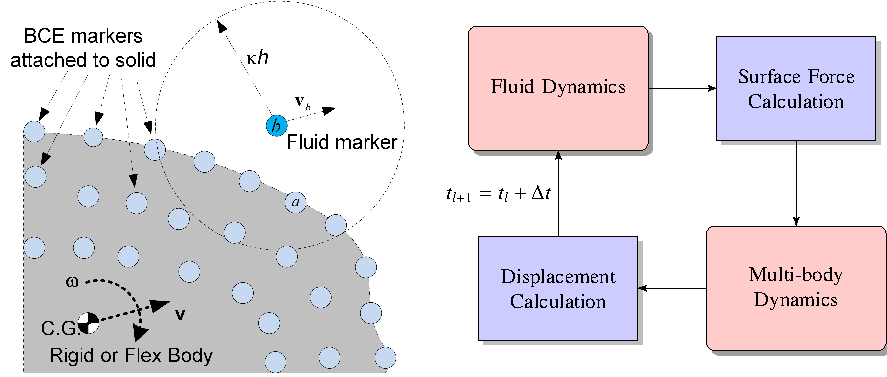
\includegraphics[width=1.\textwidth]{images/FSI.pdf}
	\end{center}
	\caption{Explicit coupling via BCE markers between a solid body, rigid or deformable (shown as the gray object), and the fluid. The BCE markers, which are placed both on the solid's surface and in a thin buffer region inside it, are used towards two ends: transfer surface forces from the fluid sub-system to the solid sub-system; and, enforce no-slip boundary conditions. The position, velocity, and acceleration of the BCE markers are dictated by the solid object that these markers are associated with via Eqs.\ref{eq:DVI_EOM_DISC:1} and~\ref{eq:ANCF_r}. The depth of the buffer that hosts BCE markers is equal to the characteristic length $\kappa h$.}
	\label{fig:fsi_FD}
\end{figure}

This approach amounts to a force-displacement coupling method. The fluid impresses interfacial forces on the solid surface and in return, registers the presence of the solid through the latter's interface location and velocity. The interaction mechanism is facilitated by Boundary Condition Enforcing (BCE) markers that are placed on a solid's surface and in a thin buffer region inside the solid (see Fig.~\ref{fig:fsi_FD}, left panel). A similar approach has been described in \cite{fourey2010,armanCompFluids2015,Hu2013}. The BCE markers are attached to the solid; their \textit{expected} motion is dictated by the motion of the solid bodies to which they belong. In the case of rigid bodies, the expected position $\mathbf{r}_i^a$ and velocity $\mathbf{v}_i^a$ of the BCE marker $a$ attached to solid $i$ are obtained from Eqs.~\ref{eq:DVI_EOM_DISC:1}-\ref{eq:DVI_EOM_DISC:5}. Note that the local position vector of marker $a$ with respect to the center of mass of body $i$; i.e., ${\bar {\bf s}}^{a}_i $, is constant in time. For flexible bodies, $\mathbf{r}_i^a$ and $\mathbf{v}_i^a$ are obtained via the interpolation (shape) functions (see for instance Eqs.~\ref{eq:ANCF_Beam_r} and \ref{eq:ANCF_Shell_r}) associated with the underlying flexible element, given that the nodal coordinates, velocities, and accelerations are passed from the solid solver to the fluid solver. For instance, for 1D and 2D elements Eq.~\ref{eq:ANCF_Beam_Shapefunctions} and Eq.~\ref{eq:ANCF_Shell_r} can be used, respectively, to obtain the updated position of marker $a$ from the nodal coordinates $ {{\bq}}^{i}(t)$ and similarly to obtain the expected velocity and acceleration from the nodal velocities  ${\dot{\bq}}^{i}(t)$ and accelerations $\ddot{\bq}^{i}(t)$, respectively. Note that the local natural coordinates $\xi$, $\eta$, and $\zeta$ of the marker attached to the flexible body are constant.

The \textit{expected} kinematic attributes of the markers, calculated from the motion of the solid phase at the location occupied by the markers, are different from their \textit{assigned} values. The latter are calculated such that the no-slip and no-penetration boundary conditions are implicitly enforced at the fluid-solid interface. The no-slip condition states that the velocity of the BCE markers should oppose the velocity of the fluid particles such that the average \textit{relative} fluid-solid velocity at the interface is zero; i.e., the average velocity at the interface is the \textit{expected} interface velocity. Herein, the \textit{induced} velocity $\hat{\mathbf{v}}_a$ at the position of marker $a$ is computed from the velocity of the fluid markers via Eq.~\ref{eq:vBCE_Adami} as
\begin{equation*} 
\hat{\mathbf{v}}_a = \frac{\sum\limits_{b \in \mathbf{F}} {\mathbf{v}_b W_{ab}}}{\sum\limits_{b \in \mathbf{F}} {W_{ab}}}.
\end{equation*}
where $\mathbf{F}$ denotes a set of fluid markers that are within the compact support of the BCE marker $a$.  The no-slip condition holds if $({\hat{\mathbf{v}}_a+\mathbf{v}_a})/2=\mathbf{v}_a^p$; in other words the \textit{assigned} velocity of marker $a$ is \cite{Adami2012}:
\begin{equation} \label{eq:no_slip}
\mathbf{v}_a = 2 \mathbf{v}^{p}_a - {\hat{\mathbf{v}}}_a.
\end{equation}
The pressure of a BCE marker is calculated via a force balance condition at the wall interface, which leads to Eq.~\ref{eq:pBCE_Adami} as follows \cite{Adami2012}
\begin{equation*}
p_a = \frac{\sum\limits_{b \in \bf F} {p_b W_{ab}} + \left( \mathbf{g} - \mathbf{a}_a^p \right) \cdot \sum\limits_{b \in \bf F} {\rho_b \mathbf{r}_{ab} W_{ab} }}{\sum\limits_{b \in \bf F} {W_{ab}}},
\end{equation*}
where $\mathbf{g}$ is the gravitational acceleration and $\mathbf{a}_a^p$ is the acceleration of the solid phase at the location of  marker $a$. The fluid-solid coupling procedure is described in Algorithm~\ref{alg:FSI}.

\begin{algorithm}[H] 
	\caption{Fluid-Solid coupling procedure. Carried out at each time step.}
	\begin{algorithmic}[1]
		\STATE The fluid phase is integrated in time.
		\STATE  The pressure and viscous forces exerted by the fluid markers on the BCE markers are obtained via
		Eqs.~\ref{eq:Fi} and \ref{eq:viscosity} for IISPH method,
		and Eq.~\ref{eq:FS_ISPH} for WCSPH and ISPH methods.
		
		
		
		\STATE The generalized forces on each rigid body or nodal coordinate are calculated by collecting the forces of their associated BCE markers.
		\STATE Generalized forces are used to solve multibody dynamics involving rigid and flexible bodies.
		\STATE The position, velocity, and acceleration of the BCE markers are updated based on the new position, velocity, and acceleration of the rigid and flexible bodies.
		\STATE The velocities and pressure of the BCE markers required for the no-slip and no-penetration conditions are obtained from Eq.~\ref{eq:vBCE_Adami} and \ref{eq:pBCE_Adami}, respectively.
	\end{algorithmic}\label{alg:FSI}
\end{algorithm}

The fluid-solid coupling strategy outlined in Algorithm~\ref{alg:FSI} will yield slight numerical artifacts at the interface in relation to incompressibility and/or satisfying no-slip/no-penetration at the end of a time-step. This is a consequence of the explicit attribute of the coupling strategy. A fully implicit coupling as provided by a monolithic solver addresses this issue albeit at an increase in run-time.  As a rule of thumb, IISPH, ISPH, and WCSPH yield expeditious solutions while a monolithic solver such as KCSPH can provide a better quality solution at the interface yet at a higher computational cost. Certainly, as the time step decreases, ISPH, IISPH and WCSPH produce increasingly more accurate solutions yet at that point, they forfeit their inexpensive-solution attribute.

\section{Viscoplasticity}
A robust and accurate numerical implementation of the yield stress in the Navier-Stokes equations is still a matter of research \cite{ragui2018progress}. The difficulty is in modeling the discontinuity arising from the yield stress; the material should only flow if the shear stress exceeds the yield stress $\tau_0$ (see Fig.~\ref{fig:HB}). In other words:
\begin{align}
\begin{cases}
\text{yielded region :}\qquad & \tau>\tau_0\\
\text{unyielded region :}\qquad& \tau<\tau_0\\
\end{cases}.
\end{align}
This discontinuity cannot be strictly handled for truly static zones in a continuum if one chooses to use a non-Newtonian approach. A more rigorous approach is to solve the time-evolution of the stress tensor besides the Navier-Stokes and the continuity equations and keeping track of the stress tensor via a linear elastic relation between the stress and strain tensors \cite{gray2001sph,Monaghan2000} to obtain the rate of shear stress as following
\begin{equation}\label{eq:shear_stress_rate}
\frac{d\sigma^{\alpha\beta}}{dt} = 2G(E^{\alpha\beta}-\frac{1}{3}\delta^{\alpha\beta}{E}^{\gamma\gamma})-\sigma^{\alpha\gamma}\omega^{\gamma\beta} + \omega^{\alpha\gamma}\sigma^{\gamma\beta},
\end{equation}
where $G$ is the shear modulus, $\vect{E}$ is the deformation gradient tensor defined in Eq.~\ref{eq:def_rate} and $\bm \omega$ is the rotation tensor defined as
\begin{align}
\bm \omega=\frac{1}{2}(\nabla\bf{u}-\nabla\bf{u}^T).
\label{eq:rot_rate}
\end{align}
This approach involves the scaling of the stress tensor back to the yield surface once the stress grows beyond the yield criteria and is the matter of an ongoing research effort. 

Amongst many simple and exponential regularization models proposed in the literature, the bi-viscosity model is chosen in this thesis. This models allows for enforcing the yield stress over a infinitesimal strain-rate range without the need for solving an equation such as Eq.~\ref{eq:shear_stress_rate}, yet has its drawbacks as mentioned earlier. The bi-viscosity model is as follows:
\begin{align}
\tau=
\begin{cases}
\tau_0+ k \dot{\gamma}^n \qquad & \dot{\gamma}>\dot{\gamma_0}\\
(\tau_0/\dot{\gamma_0})\dot{\gamma}\qquad&  \dot{\gamma}<\dot{\gamma_0}\\
\end{cases},
\end{align}
where $\mu_{\infty}=(\tau_0/\dot{\gamma_0})$ is a large value acting as a penalty viscosity. Schematics of the bi-viscosity model is demonstrated in Fig.~\ref{fig:biviscosity}. This approach although has its drawbacks, has been used widely in the literature \cite{ragui2018progress,tanner1983numerical}.
\begin{figure}[H]
	\begin{center}
		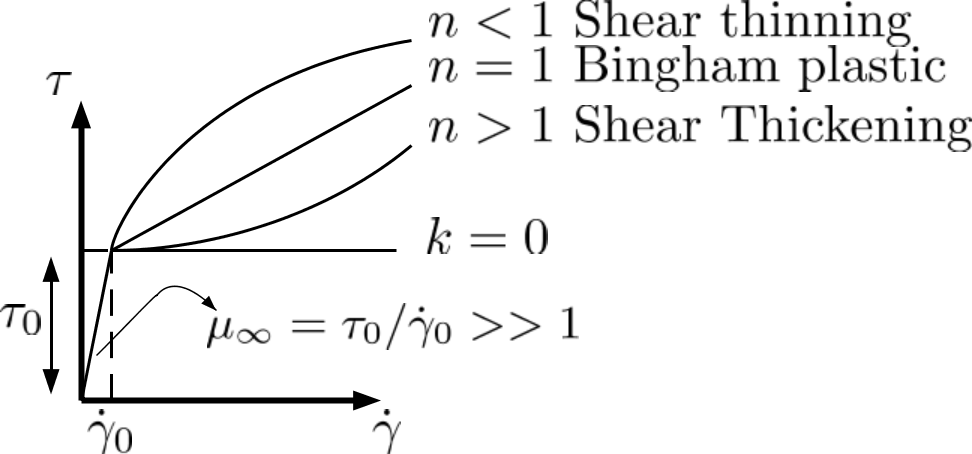
\includegraphics[width=.6\linewidth]{images/Non-newtonian-Biviscosity.png}
	\end{center}
	\caption{Numerical implementation of the yield stress using bi-viscosity model.}
	\label{fig:biviscosity}
\end{figure}

